\chapter{The geometric longitude of a tree of crossing circles}
\label{app:geometric-characteristic}\label{gi:the-geometric-longitude-of-a-tree-of-crossing-circles}

The edge equations of a tree of crossing circles determine a representation
of its link exterior. They determine the auxiliary meridians and longitudes
directly. This note identifies the main preferred longitude: its eigenvalue
is the product of the edge factors, with the monomial prescribed by the
original zero framing.

The construction retains the ordered tangles, crossing disks and their
primitive peripheral curves. The half twist at a disk is inserted through
its full two-generator boundary action. Merely exchanging three ideal
vertices while retaining the old white-face maps would give a false gluing
away from the parabolic main meridian.

This is a geometric and algebraic identification. It does not extend a
quantum asymptotic theorem to arbitrary short fillings.

\section{The diagram and the longitude identity}\label{gi:the-diagram-and-the-longitude-identity}

Take a finite tree with at least one edge. At each vertex \(v\), place
one two-strand crossing-circle tangle, whose auxiliary circle bounds
the specified twice-punctured disk. Retain a crossing
\(R^{\epsilon_v}\), with \(\epsilon_v\in\{-1,0,1\}\).
Every edge is an actual quarter-turn attachment between ordered stacks.
The product order, rotations of the tangle balls, endpoint frames and
cylindrical closing map are part of the diagram. There are no product
junctions without their own crossing circle.
Write \(\mathcal E\) for its set of edges.

The \href{https://sashakolpakov.github.io/murakamis_dream/notes/actual_all_circle_octahedral_decomposition.html}{ordered decomposition}
constructs two projection balls from this literal diagram. Each original
edge contributes two octahedra. At each circle their disk-side pages
are joined in the original cyclic order, with its retained half twist
on one distinguished seam. Assume the main strands form one component,
and orient that knot.

Let \(\mu_K\) be its positive meridian and
\(\lambda_{\mathrm{aug}}\) its preferred longitude in the augmented
exterior. Use the main eigenvalue parameter \(M\). The source flag
is the \(M^{-1}\) eigenline; the longitude coordinate below is its
inverse eigenvalue, equivalently the eigenvalue on the \(M\) line.
At auxiliary circle \(v\), the selected eigenvalue of the original
primitive disk longitude is \(-Q_v\), so its projective similarity
is \(Q_v^2\). Write \(U_v\) for the logarithm of its primitive
meridian similarity at that auxiliary flag.

For each edge \(e=vw\), introduce \(X_e\) and impose

\begin{equation}\label{gi:T1}
(X_e+Q_v)(X_e+Q_v^{-1})(X_e+Q_w)(X_e+Q_w^{-1})
       =(X_e-1)^2(1-X_eM^2)(1-X_e/M^2).
\end{equation}

Choose the branch through \(M=Q_v=1\), \(X_e=i\). Set

\begin{equation}\label{gi:T2}
\rho_{v,e}=\frac{Q_v+X_e}{1+Q_vX_e},\qquad
 f_e=\frac{M^2-X_e}{1-M^2X_e}.
\end{equation}

All rational identities are read on their regular open sets and then
continued on the same irreducible source variety. Clearing a denominator
does not add a new geometric branch.

\textbf{Theorem.} Equations \eqref{gi:T1} give a representation of the original
augmented exterior near its marked complete structure. Its primitive
auxiliary similarities are

\begin{equation}\label{gi:T3}
\exp U_v=Q_v^{-\epsilon_v}
                                  \prod_{e\ni v}\rho_{v,e}.
\end{equation}

If \(w_\epsilon\) is the oriented writhe of the retained crossings and
\(a_{\mathrm{aug}}=-w_\epsilon-\sum_v\epsilon_v\), then

\begin{equation}\label{gi:T4}
L_{\mathrm{aug}}^2
                     =M^{2a_{\mathrm{aug}}}\prod_e f_e^2.
\end{equation}

Fill circle \(v\) on its original primitive slope
\(\mu_v+p_v\lambda_v\), with
\(n_v=\epsilon_v-2p_v\). The exponentiated filling equations are

\begin{equation}\label{gi:T5}
\prod_{e\ni v}\rho_{v,e}=Q_v^{n_v}.
\end{equation}

Where \(Q_v^2\ne1\) for every filled circle, these equations make
each filling word projectively trivial, so the representation factors
through the filled group. On that locus its preferred longitude satisfies

\begin{equation}\label{gi:T6}
L_{\mathrm{fill}}^2=M^{2a(D)}\prod_e f_e^2,\qquad
                        a(D)=-w(D)-\sum_v n_v.
\end{equation}

Here \(w(D)\) is the writhe of the original filled diagram.
The squared formula is also an identity for the corresponding peripheral
word on the augmented source variety. At \(Q_v=\pm1\), equation \eqref{gi:T5}
alone need not kill a nontrivial parabolic filling word, so that word
identity does not by itself give a representation of the filled group.

On a connected germ anchored at a complete hyperbolic filled knot
point supplied by the existing marked completion theorem, the
determinant-one sign is fixed:

\begin{equation}\label{gi:T7}
\boxed{\displaystyle
       L_{\mathrm{fill}}
          =-M^{a(D)}\prod_e\frac{M^2-X_e}{1-M^2X_e}.}
\end{equation}

This is the geometric longitude of the original knot complement.
It uses its preferred meridian and longitude; it is not a longitude
of a different comparison diagram.

The complete anchor and the primitive logarithmic filling marks are
retained in Section~\ref{gi:the-complete-anchor-and-the-primitive-filling-equations}. The proof first establishes the squared
identity, without a choice of global determinant-one lift, and then
fixes the sign by a Seifert-surface frame calculation in Section~\ref{gi:the-determinant-one-sign-at-the-complete-filled-knot}.
The algebraic constant-field lemma also holds for finite simple graphs;
the geometric theorem here is restricted to the literal ordered trees.

\section{The local face maps}\label{gi:the-local-face-maps}

We first construct the two-octahedron piece with its original
white and shaded face labels. In this section \(E_0\) is a preliminary
white-face coordinate, and \(X\) is the edge variable in \eqref{gi:T1}.
Their distinction matters when \(M\ne1\).

\subsection{The parameters and the actual faces}\label{gi:the-parameters-and-the-actual-faces}

Write \(M\) for the main meridian eigenvalue parameter and set
\(m=M^2\). The symbols \(Q\) and \(P\) are the chosen square roots
of the two auxiliary longitude similarities. All parameters are near
\((m,Q,P)=(1,1,1)\). We use \(E_0\) for a white-face
coordinate, near \(i\). The effective-action wire coordinate will be
denoted \(X\).

The two projection copies have six ideal vertices

\begin{equation}\label{gi:N1}
\begin{array}{c|c|c}
 &\text{equator}&\text{circle apices}\\ \hline
 +&(0,\infty,1,R)&(A,B)\\
 -&(0,\infty,1,S)&(a,b).
 \end{array}
\end{equation}

The four white identifications are the unique maps of the ordered
triangles

\begin{equation}\label{gi:N2}
\begin{aligned}
 W_0:(A,0,\infty)&\longmapsto(a,0,\infty),&
 W_1:(B,\infty,1)&\longmapsto(b,\infty,1),\\
 W_2:(A,1,R)&\longmapsto(a,1,S),&
 W_3:(B,R,0)&\longmapsto(b,S,0).
\end{aligned}
\end{equation}

These are the face labels of the original two-leaf cut. Changing the
minus equator from \(R\) to \(S\) is necessary: retaining the old
four white matrices would keep all four main meridians parabolic.

Put \(L=E_0^{-1}\), and define

\begin{equation}\label{gi:N3}
\begin{gathered}
 S=\frac{m^2R}{1+(m^2-1)R},\qquad
 \ell_1=L/m,\quad \ell_2=L/m^2,\quad \ell_3=Lm,\\
 c_2=\frac{\ell_2(R-1)/(S-1)-1}{R-1},\qquad
 c_3=\frac{\ell_3R/S-1}{R},\\
 W_0=\begin{pmatrix}L&0\\0&1\end{pmatrix},\quad
 W_1=\begin{pmatrix}\ell_1&1-\ell_1\\0&1\end{pmatrix},\\
 W_2=\begin{pmatrix}c_2+\ell_2&1-c_2-\ell_2\\c_2&1-c_2\end{pmatrix},
 \qquad
 W_3=\begin{pmatrix}\ell_3&0\\c_3&1\end{pmatrix}.
\end{gathered}
\end{equation}

Thus \(W_2(z)=1+\ell_2(z-1)/(1+c_2(z-1))\).
Every map sends its two equatorial vertices in \eqref{gi:N2} correctly.

If \(q=(0,\infty,1,R)\), the native main corner word
\(W_{j-1}^{-1}W_j\) fixes \(q_j\) and has local derivative

\begin{equation}\label{gi:N4}
(m^{-1},m,m^{-1},m)_j.
\end{equation}

At infinity the local coordinate is \(1/z\). To derive \eqref{gi:N3},
start with \(W_0(z)=Lz\). The derivatives at infinity, 1 and 0
give respectively \(\ell_1=L/m,\ell_2=L/m^2,\ell_3=Lm\).
The remaining derivative at \(R\), on its branch through the
complete chart, gives the displayed formula for \(S\).
This supplies the actual peripheral condition, not just equal traces.

\subsection{The auxiliary longitude equations and the local gluing locus}\label{gi:the-auxiliary-longitude-equations-and-the-local-gluing-locus}

Take

\begin{equation}\label{gi:N5}
A=\frac{mE_0+Q}{m+Q},\qquad B=\frac{P(1-mE_0)}{P+m},\qquad
 a=A/E_0,\qquad b=1+\frac{B-1}{E_0m}=-\frac{B}{E_0P}.
\end{equation}

There are two expressions for the equatorial coordinate:

\begin{equation}\label{gi:N6}
\begin{aligned}
 R_v&=\frac{(mE_0+Q)(mE_0Q+1)}
 {E_0m(Q^2+1)+2E_0Qm^2+Q(1-m^2)},\\
 R_w&=-\frac{P(mE_0-1)^2}
 {E_0m^2(P^2+1)+2E_0Pm+P(m^2-1)}.
\end{aligned}
\end{equation}

The first is exactly \(W_2(A)=a\); the second is exactly
\(W_3(B)=b\). Their common value is \(R\).

For completeness, the longitude choices made here can be obtained
before solving for the apices. The first longitude is
\(W_2^{-1}W_0\). Its similarity in the coordinate with \(A\)
at infinity is \(W_2'(A)/L\), and is prescribed as \(Q^2\).
The chosen square-root branch is
\(1+c_2(A-1)=-1/(mQ)\). At the other circle the longitude is
\(W_1^{-1}W_3\), with similarity
\(\ell_1/W_3'(B)=P^2\), and the chosen branch is
\(1+c_3B=-mP\). Substitution gives \eqref{gi:N5}--\eqref{gi:N6}.
Both signs equal \(-1\) at completeness.

Clearing the nonzero denominators of \(R_v-R_w\), and removing
the factor \(E_0m^2\), gives

\begin{equation}\label{gi:N7}
\begin{aligned}
G={}&E_0^2P^2Qm^2+E_0^2PQ^2m+2E_0^2PQm^2+2E_0^2PQm
       +E_0^2Pm+E_0^2Qm^2\\
 &+E_0P^2Q^2m+E_0P^2m-4E_0PQm+E_0Q^2m+E_0m\\
 &+P^2Q+PQ^2m+2PQm+2PQ+Pm+Q.
\end{aligned}
\end{equation}

The local gluing equation is \(G=0\). At \(m=Q=P=1\),
\(G=8(E_0^2+1)\), so \(G_{E_0}(i,1,1,1)=16i\).
It follows that there is a unique holomorphic branch \(E_0\) near
\(i\). Every denominator displayed above is nonzero on a sufficiently
small neighborhood of this branch.

The pure shaded maps in the two plus-copy circle frames are

\begin{equation}\label{gi:N8}
S_v(A,R)=
 \begin{pmatrix}0&RA(1-A)\\A-R&R-A^2\end{pmatrix},\qquad
 S_w(B,R)=
 \begin{pmatrix}B(B-1)&-RB(B-1)\\B-R&R-B\end{pmatrix}.
\end{equation}

The first fixes \(A\) and sends \(\infty\) to \(0\) and \(1\)
to \(R\). The second fixes \(B\) and sends \(R\) to \(0\)
and \(1\) to infinity. The minus maps are the same formulas with
\((A,B,R)\) replaced by \((a,b,S)\); denote them by
\(S_v^-\) and \(S_w^-\).

All the actual white/shaded edge returns hold projectively:

\begin{equation}\label{gi:N9}
\begin{array}{lll}
 W_0S_v=S_v^-W_0,&W_2S_v=S_v^-W_2,&W_3S_v=S_v^-W_1,\\
 W_1S_w=S_w^-W_1,&W_3S_w=S_w^-W_3,&W_0S_w=S_w^-W_2.
\end{array}
\end{equation}

The first row follows already on \(R=R_v\), and the second on
\(R=R_w\). One can verify each equality by multiplying one side
by the adjugate of the other: both off-diagonal entries and the
diagonal difference vanish. Consequently these are the face maps
of the marked local representation of the original cut, rather than
maps chosen solely to reproduce a character polynomial.

At completeness their apices are

\begin{equation}\label{gi:N10}
(A,B)=((1+i)/2,(1-i)/2),\quad
 (a,b)=((1-i)/2,(1+i)/2),\quad R=S=1/2.
\end{equation}

The eight ordered tetrahedral shapes of the original apical
subdivision are then \(i\). Holomorphic continuity preserves their
positive imaginary parts on a sufficiently small parameter
neighborhood. This is a local incomplete hyperbolic structure with
decorated main eigenflags; it does not assert completeness at a
nonparabolic main cusp.

\subsection{The wire coordinate is determined by the actual meridian}\label{gi:the-wire-coordinate-is-determined-by-the-actual-meridian}

The positively chosen auxiliary meridians are \(S_v^{-1}\) and
\(S_w^{-1}\). Sending the corresponding apex to infinity changes
their similarities into the ordinary derivatives of \(S_v,S_w\)
at those apices. Direct differentiation of \eqref{gi:N8} gives

\begin{equation}\label{gi:N11}
\begin{aligned}
 U_v^{\exp}
 &=-\frac{A(A-R)}{R(1-A)}
   =\frac{(E_0m+Q)(Qm+1)}{(Q+m)(E_0Qm+1)},\\
 U_w^{\exp}
 &=\frac{B(R-1)}{(B-R)(B-1)}
   =\frac{(E_0+P)(P+m)}{(E_0P+1)(Pm+1)}.
\end{aligned}
\end{equation}

These are similarities of the primitive words, not the squares of
unrecorded primitive words. The actual longitude similarities are
exactly \(Q^2,P^2\), as established in Section~\ref{gi:the-auxiliary-longitude-equations-and-the-local-gluing-locus}.

Solve \(U_v^{\exp}=(Q+X)/(1+QX)\) for \(X\).
Cancel the removable \(Q=1\) factor before taking that limit:

\begin{equation}\label{gi:N12}
X=
 \frac{E_0Q^2m+E_0Qm^2+E_0Qm+E_0m-Qm+Q}
 {E_0Qm^2-E_0Qm+Q^2m+Qm+Q+m}.
\end{equation}

The denominator is \(4\) at completeness. The second meridian
similarly gives

\begin{equation}\label{gi:N13}
X_w=-\frac{E_0P^2m+E_0Pm+E_0P+E_0m+Pm-P}
 {E_0Pm-E_0P-P^2-Pm-P-1}.
\end{equation}

Their difference is \((m-1)G\) divided by the product of the
two displayed denominators. Hence \(X=X_w\) on the actual
gluing locus. In particular

\begin{equation}\label{gi:N14}
U_v^{\exp}=\frac{Q+X}{1+QX},\qquad
 U_w^{\exp}=\frac{P+X}{1+PX},\qquad X|_{m=1}=E_0.
\end{equation}

Thus the same source wire variable is selected from both actual
auxiliary meridians.

Substitution of \eqref{gi:N12} and \eqref{gi:N7} now gives

\begin{equation}\label{gi:N15}
(X+Q)(X+Q^{-1})(X+P)(X+P^{-1})
       =(X-1)^2(1-Xm)(1-X/m).
\end{equation}

For a direct polynomial check, after reducing the rational
expression its numerator is \(G\) times
\[
 (Q+1)^2(Q+m)(Qm+1)
       (E_0Q^2m+E_0Qm^2+E_0Qm+E_0m-Qm+Q).
\]
Nonzero unit factors can differ if the common denominator is not
reduced. Alternatively put
\(\mathcal A=X+X^{-1}\), \(\mathcal B=Q+Q^{-1}\),
\(\mathcal C=P+P^{-1}\), \(\mathcal D=m+m^{-1}\).
Equation \eqref{gi:N15} is

\begin{equation}\label{gi:N16}
(\mathcal A+\mathcal B)(\mathcal A+\mathcal C)
  =(\mathcal A-2)(\mathcal A-\mathcal D),\qquad
 \mathcal A=\frac{2\mathcal D-\mathcal B\mathcal C}
                  {\mathcal B+\mathcal C+\mathcal D+2}.
\end{equation}

The denominator in the last expression is \(8\) at completeness.
This is the effective edge equation with \(m=M^2\).

\subsection{The full disk-side seam, including its main punctures}\label{gi:the-full-disk-side-seam-including-its-main-punctures}

Use the ordered cross ratio
\([a,b,c,d]=(a-c)(b-d)/((a-d)(b-c))\).
The incoming plus-copy triangle at the first circle is
\((A,\infty,1)\); the outgoing triangle is \((A,R,0)\).
Develop the adjacent minus triangle back through its actual white
map. The six neighboring third vertices are respectively

\begin{equation}\label{gi:N17}
E_0,\quad W_1^{-1}(a),\quad W_2^{-1}(\infty),\qquad
 W_2^{-1}(0),\quad W_3^{-1}(a),\quad W_0^{-1}(S).
\end{equation}

Substituting \eqref{gi:N3}--\eqref{gi:N6}, with \(R=R_v\), gives

\begin{equation}\label{gi:N18}
\begin{array}{c|ccc}
 \text{incoming edge}&(A,\infty)&(\infty,1)&(1,A)\\ \hline
 \text{ratio}&-m/Q&-Q&-1/(mQ)\\
 \text{outgoing edge}&(A,R)&(R,0)&(0,A)\\ \hline
 \text{ratio}&-mQ&-1/Q&-Q/m .
\end{array}
\end{equation}

For example, the first ratio is \((A-1)/(A-E_0)=-m/Q\).
The other five reduce by the same single substitution. In particular
the table is independent of the other circle parameter \(P\) and
of the preliminary wire coordinate \(E_0\).

The original pure disk-side matching reverses the two main
punctures: outgoing \((A,R,0)\) is identified with incoming
\((A',1,\infty)\). Thus the outgoing entries are paired with
the incoming entries in reverse order. Each resulting product is
one, including its complex shear. A map of the three ordered
vertices identifies the first triangles; the three ratios then
identify the adjacent second triangles. This proves equality of
the full marked two-triangle disk-side structures. It does not
replace that matching by an arbitrary pants permutation.

The main puncture multipliers visible in the incoming table are
\(m,m^{-1}\), and the circle multiplier is \(Q^{-2}\);
the outgoing table reverses the boundary orientation. These
multipliers explain why recording the puncture order is essential.
Replacing \(M\) by \(M^{-1}\) exchanges eigenflags and is not
an innocuous reset of the marked representation.

Consequently any chain of these \emph{compatibly framed pure seams}
can be sewn in its original cyclic order. The geometric seam at
each step uses the same \(m,Q\); it requires no parameter from
the opposite end of an edge. Products of the auxiliary meridian
increments are therefore products of the factors in \eqref{gi:N14}.
The actual main component and its globally positive meridian
must still be traced through the endpoint frames, as explained
in Section~\ref{gi:ordered-pages-and-the-half-twist-collar} below.

\section{A regular character chart for the same piece}\label{gi:a-regular-character-chart-for-the-same-piece}

The face chart identifies the actual topology. The following rational
matrix chart is useful both for its peripheral words and for continuation
to generic auxiliary values over any fixed \(M\ne0\).
Throughout this section use

\begin{equation}\label{gi:C0}
\begin{gathered}
 t=M+M^{-1},\quad D=M^2+M^{-2}=t^2-2,\\
 \beta=Q+Q^{-1},\quad\gamma=P+P^{-1},\\
 A_0=X+X^{-1},\quad S=\beta+\gamma+t^2.
 \end{gathered}
\end{equation}

Equation \eqref{gi:T1} is

\begin{equation}\label{gi:C0a}
(A_0+\beta)(A_0+\gamma)=(A_0-2)(A_0-D),\qquad
 A_0=\frac{2D-\beta\gamma}{S}.
\end{equation}

The denominator is eight at completeness. In the following matrix
formulas the internal mixed trace is denoted \(\mathcal X\), so it
is distinct from the source wire \(X\).

\subsection{A four-puncture character and its explicit matrices}\label{gi:a-four-puncture-character-and-its-explicit-matrices}

Put

\begin{equation}\label{gi:C5}
p=-\beta,\qquad q=-\gamma,\qquad \mathcal X=2+SX,
 \qquad b=p-2,\quad h=M-M^{-1}.
\end{equation}

For the moment \(p,q,\mathcal X\) may be arbitrary nearby parameters. Define

\begin{equation}\label{gi:C6}
A=\begin{pmatrix}M&1\\0&M^{-1}\end{pmatrix},
 \qquad
 B=\begin{pmatrix}M^{-1}&0\\b&M\end{pmatrix}.
\end{equation}

Both have determinant one and trace \(t\), and \(\operatorname{tr}(AB)=p\). Set

\begin{equation}\label{gi:C7}
\begin{gathered}
 c=\frac{M\mathcal X+M^{-1}q-2t}{D-p},\qquad
 d=\frac{q-M^2-1+hc}{p-2},\\
 e=\mathcal X-1-M^{-2}-hc,\qquad
 C=\begin{pmatrix}c&d\\e&t-c\end{pmatrix}.
 \end{gathered}
\end{equation}

The denominators \(p-2=-4\) and \(D-p=4\) at the complete point are nonzero. The construction does not divide by \(M-M^{-1}\). Direct multiplication gives

\begin{equation}\label{gi:C8}
\operatorname{tr}C=t,\qquad
 \operatorname{tr}(BC)=q,\qquad
 \operatorname{tr}(AC)=\mathcal X,\qquad
 \operatorname{tr}(ABC)=t.
\end{equation}

For the last identity, the nonconstant part of the trace is
\(bc+Me+M^{-1}bd\), which vanishes by \eqref{gi:C7}.

The determinant calculation is

\begin{equation}\label{gi:C9}
\det C-1=\frac{\mathcal F(\mathcal X,p,q)}{(p-2)(D-p)},
\end{equation}

where

\begin{equation}\label{gi:C10}
\mathcal F=
 \mathcal X^2+p^2+q^2+pq\mathcal X-2t^2(p+q+\mathcal X)+4t^2+t^4-4.
\end{equation}

This is the equal-boundary-trace four-punctured-sphere character equation, derived here from the matrices. For a direct verification of \eqref{gi:C9}, substitute the three entries in \eqref{gi:C7}, multiply by \((p-2)(D-p)\), and collect the quadratic polynomial in \(\mathcal X\). Its leading coefficient is one; the other two coefficients are those displayed in \eqref{gi:C10}.

Now impose \eqref{gi:C5}. A direct substitution gives the especially simple identity

\begin{equation}\label{gi:C11}
\mathcal F(2+SX,-\beta,-\gamma)
 =XS\bigl[(A_0+\beta)(A_0+\gamma)
                         -(A_0-2)(A_0-D)\bigr].
\end{equation}

Thus \eqref{gi:T1} is equivalent to \(\det C=1\) on this regular chart. Put

\begin{equation}\label{gi:C12}
D_0=(ABC)^{-1}.
\end{equation}

Equations \eqref{gi:C8}--\eqref{gi:C12} give

\begin{equation}\label{gi:C13}
ABCD_0=I,\qquad
 \det A=\det B=\det C=\det D_0=1,\qquad
 \operatorname{tr}A=\operatorname{tr}B
       =\operatorname{tr}C=\operatorname{tr}D_0=t.
\end{equation}

These are literal matrices representing the four positively oriented boundary generators of a four-punctured sphere. Each puncture has eigenvalues \(M,M^{-1}\). In particular, the source relation is not merely similar in degree to a character equation: \eqref{gi:C7}, \eqref{gi:C11}, and \eqref{gi:C12} realize it by actual matrices.

At the complete selected point,

\begin{equation}\label{gi:C14}
A=\begin{pmatrix}1&1\\0&1\end{pmatrix},\quad
 B=\begin{pmatrix}1&0\\-4&1\end{pmatrix},\quad
 C=\begin{pmatrix}-1+2i&1\\8i&3-2i\end{pmatrix}.
\end{equation}

All four punctures are noncentral parabolics. The pair \(A,B\) has no common eigenline. The construction is therefore on a regular irreducible character chart through the complete point.

The alternative root of the quadratic \eqref{gi:C10} is \(2+S/X\). Indeed its sum with \(\mathcal X=2+SX\) is \(2t^2-\beta\gamma\), by \eqref{gi:C0a}. For comparison, its discriminant factors as

\begin{equation}\label{gi:C15}
(\beta+2)(\gamma+2)
       \bigl[\beta\gamma-2\beta-2\gamma-4D-4\bigr]
           =S^2(X-X^{-1})^2.
\end{equation}

This verifies the two-sheeted parameter and its branch without assigning signs by a numerical square root.

\subsection{Auxiliary transport matrices with the actual source ratios}\label{gi:auxiliary-transport-matrices-with-the-actual-source-ratios}

Define two invertible projective transport matrices

\begin{equation}\label{gi:C16}
V=AB+z_v I,\qquad T=BC+z_w I,
 \qquad
 z_v=-\frac{1+X(\beta+1)}{1-X},\qquad
 z_w=\frac{X+\gamma+1}{1-X}.
\end{equation}

Scalar multiples of \(V,T\) give the same projective transports. Their determinant-one normalizations can be chosen on a local square-root cover; every commutator below is independent of that choice.

The following full matrix identities hold on \eqref{gi:T1}:

\begin{equation}\label{gi:C17}
\begin{aligned}
 VA&=D_0^{-1}V,& VB&=C^{-1}V,\\
 TB&=A^{-1}T,& TC&=D_0^{-1}T.
 \end{aligned}
\end{equation}

They are stronger than trace matching. Also \(V\) commutes with \(AB\), and \(T\) commutes with \(BC\), directly from \eqref{gi:C16}.

Here is a rational way to verify \eqref{gi:C17}, preserving the regular chart. Eliminate \(\gamma\) using \eqref{gi:C0a}:

\begin{equation}\label{gi:C18}
\gamma=\frac{2D-(X+X^{-1})(\beta+D+2)}
                         {X+X^{-1}+\beta}.
\end{equation}

The denominator is two at the complete point. Substitute \eqref{gi:C18}, \eqref{gi:C5}, and \eqref{gi:C7} in \eqref{gi:C17}. Every difference becomes a zero rational function of \(M,\beta,X\). This is also a polynomial certificate after clearing the recorded denominators. For example, before substituting \eqref{gi:C5}, the value of \(z\) solving the lower-left entry of
\((AB+zI)A=(ABC)(AB+zI)\) makes the remaining three entries scalar multiples of \eqref{gi:C10}; after \eqref{gi:C5}, that \(z\) reduces to \(z_v\). The other pair follows by cyclic permutation of the four punctures. No eigenline diagonalization at a repeated eigenvalue is used.

The two disk-longitude words and their selected eigenvalues are

\begin{equation}\label{gi:C19}
\Lambda_v=AB,\quad \lambda_v=-Q;
 \qquad
 \Lambda_w=(BC)^{-1},\quad \lambda_w=-P.
\end{equation}

The inverse in the second word records the opposite boundary orientation. On the \(-Q\) eigenline of \(AB\), the projective eigenvalue ratio of \(V\) is

\begin{equation}\label{gi:C20}
\frac{z_v-Q}{z_v-Q^{-1}}
                         =\frac{Q+X}{1+QX}.
\end{equation}

This identity follows by factoring the numerator as
\(-(1+Q)(1+X/Q)/(1-X)\) and the denominator as
\(-(1+Q^{-1})(1+XQ)/(1-X)\).

For \(T\), note \(z_w=z_v(P,X^{-1})\). Its ratio on the \(-P\) eigenline of \(BC\) is therefore the inverse of \((P+X)/(1+PX)\). The selected eigenline of \(\Lambda_w=(BC)^{-1}\) with eigenvalue \(-P\) is instead the \(-P^{-1}\) eigenline of \(BC\). Thus its marked ratio is

\begin{equation}\label{gi:C21}
\frac{z_w-P^{-1}}{z_w-P}
                         =\frac{P+X}{1+PX}.
\end{equation}

Equations \eqref{gi:C20}--\eqref{gi:C21} are exactly the two source auxiliary ratios. Their extension to \(Q=P=1\) is the full matrix limit of \eqref{gi:C16}, not a separate evaluation of two coalescing eigenvectors.

The determinants are nonzero nearby. More explicitly, after \eqref{gi:C18},

\begin{equation}\label{gi:C22}
\begin{aligned}
 \det V&=\frac{(\beta+2)(\beta X+X^2+1)}{(X-1)^2},\\
 \det T&=
 -\frac{(X-1)^2(X-M^2)(XM^2-1)
                (\beta M^2+M^4+1)}
 {M^4(\beta X+X^2+1)^2}.
 \end{aligned}
\end{equation}

Both equal \(-4\) at the complete point. These formulas fix the regularity needed for the inverse transport matrices.

\subsection{The main commutator gives the source longitude factor}\label{gi:the-main-commutator-gives-the-source-longitude-factor}

Consider the ordered commutator

\begin{equation}\label{gi:C23}
\Lambda_K=T V^{-1}T^{-1}V.
\end{equation}

It commutes with \(A\). This also follows from the transport paths: its inverse \(V^{-1}TVT^{-1}\) sends \(A\) successively to \(B^{-1}\), \(C\), \(D_0^{-1}\), and back to \(A\), using \eqref{gi:C17}.

Set

\begin{equation}\label{gi:C24}
u=\frac{M^2-X}{1-M^2X}.
\end{equation}

The exact matrix is

\begin{equation}\label{gi:C25}
\Lambda_K=
 \begin{pmatrix}
 -u & (u^{-1}-u)/(M-M^{-1})\\
 0  & -u^{-1}
 \end{pmatrix}.
\end{equation}

The apparent quotient in its upper-right entry is removable at \(M=1\). A direct certificate, without multiplying four complicated inverse matrices, is

\begin{equation}\label{gi:C26}
T V=V
 \begin{pmatrix}
 -u^{-1}&(u-u^{-1})/(M-M^{-1})\\
 0&-u
 \end{pmatrix}T.
\end{equation}

Substitution of \eqref{gi:C7}, \eqref{gi:C16}, and \eqref{gi:C18} makes every entry of the difference zero. Multiplication by \(V^{-1}\) and \(T^{-1}\), which are legitimate by \eqref{gi:C22}, gives \eqref{gi:C25}. The expression for the upper-right entry is regular because \(u=1\) at \(M=1\).

The \(M\) eigenline of the positively oriented puncture \(A\) is the first coordinate line. Thus the eigenvalue of \eqref{gi:C23} on that line is \(-u\), exactly the source factor for one edge. The original source cut selects the opposite \(M^{-1}\) eigenline; its eigenvalue is \(-u^{-1}\), retaining the required inverse-flag convention.

Write \(X=e^{2\pi i x}\), using the logarithm selected by \(x=1/4\)
at the complete edge. At \(M=1\), with \(X\) kept on its continued branch,

\begin{equation}\label{gi:C27}
\Lambda_K=
 \begin{pmatrix}
 -1&-2i\cot(\pi x)\\0&-1
 \end{pmatrix}.
\end{equation}

Since \(A\) translates by one, \eqref{gi:C27} has projective translation
\(2i\cot(\pi x)\). At the complete edge \(x=1/4\), this is \(2i\).
The negative SL lift in \eqref{gi:C25} is therefore compatible with the complete preferred lift; it was not inserted by multiplying the commutator by a sign.

\subsection{Comparison with the explicit native pure block}\label{gi:comparison-with-the-explicit-native-pure-block}

The face construction in Section~\ref{gi:the-local-face-maps} supplies the geometric marking
for these character matrices. The comparison retains the original
white-map order and all six white/shaded returns. Section~\ref{gi:ordered-pages-and-the-half-twist-collar} then
assembles the ordered tree and its odd seams.

Write its four actual white maps as \(W_0,W_1,W_2,W_3\), and its two plus-copy shaded maps as \(S_v,S_w\). The equatorial corners are \(0,\infty,1,R\). Put

\begin{equation}\label{gi:C28}
N_j=W_{j-1}^{-1}W_j,\qquad j\bmod4.
\end{equation}

The native corner maps have derivatives
\((M^{-2},M^2,M^{-2},M^2)\) in the finite local coordinates, with \(1/z\) at infinity. They obey
\(N_0N_1N_2N_3=I\) by literal cancellation of the white maps.

In the matrix representatives fixed in that construction,

\begin{equation}\label{gi:C29}
\det W_0=L,\quad \det W_1=L/M^2,\quad
 \det W_2=L/M^4,\quad \det W_3=LM^2.
\end{equation}

The determinant-one puncture matrices to compare with \eqref{gi:C6}--\eqref{gi:C13} are therefore

\begin{equation}\label{gi:C30}
A_{\mathrm g}=M^{-3}N_3,\quad
 B_{\mathrm g}=MN_0,\quad
 C_{\mathrm g}=MN_1,\quad
 D_{\mathrm g}=MN_2.
\end{equation}

Their product is one, since the four displayed scalar powers multiply to one. Each trace is \(M+M^{-1}\): its eigenvalue ratio is prescribed by the native corner derivative, its determinant is one, and its trace tends to \(2\) at completeness. Thus the sign is fixed by continuity, rather than reset on a puncture independently.

The two disk words now agree with their actual geometric words, including their determinant-one lifts:

\begin{equation}\label{gi:C31}
A_{\mathrm g}B_{\mathrm g}=M^{-2}W_2^{-1}W_0,\qquad
 (B_{\mathrm g}C_{\mathrm g})^{-1}
                         =M^{-2}W_1^{-1}W_3.
\end{equation}

These are the native \(v,w\) longitudes. Their selected eigenvalues are \(-Q,-P\), with their actual apex flags. The inverse in the second abstract word is essential to \eqref{gi:C31}.

\subsubsection{Actual auxiliary transports and character normalization}\label{gi:actual-auxiliary-transports-and-character-normalization}

The native shaded paths send the corners as follows:

\begin{equation}\label{gi:C32}
S_v:\infty\mapsto0,\quad 1\mapsto R;\qquad
 S_w:R\mapsto0,\quad 1\mapsto\infty.
\end{equation}

Their six white/shaded return identities imply, for the native punctures, that these paths reverse the oriented small boundary meridian at each endpoint. Thus

\begin{equation}\label{gi:C33}
\begin{aligned}
 S_vC_{\mathrm g}S_v^{-1}&=B_{\mathrm g}^{-1},
 &S_vD_{\mathrm g}S_v^{-1}&=A_{\mathrm g}^{-1},\\
 S_wA_{\mathrm g}S_w^{-1}&=B_{\mathrm g}^{-1},
 &S_wD_{\mathrm g}S_w^{-1}&=C_{\mathrm g}^{-1}.
 \end{aligned}
\end{equation}

For example, the projective relation \(W_3S_v\sim S_v^-W_1\), together with
\(W_0S_v\sim S_v^-W_0\), gives
\[
 S_v(W_0^{-1}W_1)S_v^{-1}\sim W_0^{-1}W_3=N_0^{-1}.
\]
The native matrix representatives can differ by a nonconstant scalar in this calculation; those scalars are not set to one. Normalize the punctures using \eqref{gi:C30}. The two sides now have determinant one and trace \(t\), so their projective equality has scalar \(+1\), since \(t\ne0\) near completeness. The remaining three identities follow from the other returns in the same way. This proves the literal determinant-one identities \eqref{gi:C33} without discarding a projective scalar.

Consequently

\begin{equation}\label{gi:C34}
V_{\mathrm g}=S_v^{-1},\qquad
                       T_{\mathrm g}=S_w^{-1}
\end{equation}

satisfy exactly \eqref{gi:C17}. These are the actual positively marked auxiliary meridians of the native construction, not extra operators inserted into the tangle.

There is a regular marked conjugacy to the character coordinates. At completeness the selected \(M\)-eigenlines of \(A_{\mathrm g},B_{\mathrm g}\) are distinct. Their eigenlines vary holomorphically: the matrices minus their specified eigenvalue have rank one with a nonzero entry near the parabolic point. Send those two eigenlines to infinity and zero, then fix the residual diagonal conjugation by setting the upper-right entry of \(A\) to one. This entry is a unit near completeness. The pair becomes exactly \eqref{gi:C6}, since \(\operatorname{tr}(AB)=-\beta\) fixes \(b=-\beta-2\).

The remaining matrix \(C\) is then determined by its trace, the two mixed traces, and \(\operatorname{tr}(ABC)=t\), giving \eqref{gi:C7}. The common centralizer of this irreducible pair consists only of scalars. Hence a transport satisfying \eqref{gi:C17} is unique projectively: the ratio of two such transports commutes with both punctures. Its marked eigenvalue ratio is therefore \eqref{gi:C20}, not a new free parameter.

The branch is fixed by the literal complete matrices. Substituting the complete native white maps gives
\(A_{\mathrm g}=\left(\begin{smallmatrix}3-2i&-1+i\\4-4i&-1+2i\end{smallmatrix}\right)\)
and
\(C_{\mathrm g}=\left(\begin{smallmatrix}1&-1+i\\0&1\end{smallmatrix}\right)\).
Their product has trace \(2+8i\). Since \(S=8\), the character coordinate \((\operatorname{tr}(A_{\mathrm g}C_{\mathrm g})-2)/S\) is \(i\), not the inverse root.

Let \(X_{\mathrm g}\) denote the native source wire extracted from its actual auxiliary meridian:

\begin{equation}\label{gi:C35}
U_v^{\exp}=\frac{Q+X_{\mathrm g}}{1+QX_{\mathrm g}}.
\end{equation}

The character coordinate \(X\) has the same ratio by \eqref{gi:C20}. For \(Q^2\ne1\), the fractional-linear map in \eqref{gi:C35} is injective, so \(X=X_{\mathrm g}\). Holomorphic continuation establishes equality through \(Q=1\). Equivalently,

\begin{equation}\label{gi:C36}
\operatorname{tr}(A_{\mathrm g}C_{\mathrm g})
       =2+\bigl[\beta+\gamma+(M+M^{-1})^2\bigr]X_{\mathrm g}.
\end{equation}

This proves the matching branch, rather than choosing the inverse root because the two have the same discriminant.

\subsubsection{Main basepoint, selected flag, and negative lift}\label{gi:main-basepoint-selected-flag-and-negative-lift}

The native geometric longitude based at infinity is

\begin{equation}\label{gi:C37}
\Lambda_\infty=S_wS_v^{-1}S_w^{-1}S_v.
\end{equation}

Its positively oriented main meridian is \(C_{\mathrm g}=MN_1\). In the native chart it is exactly

\begin{equation}\label{gi:C38}
C_{\mathrm g}=
 \begin{pmatrix}
 M^{-1}&M E_0-M^{-1}\\0&M
 \end{pmatrix},
\end{equation}

where \(E_0\) is the native white-face coordinate. Thus infinity is its actual \(M^{-1}\) source flag. The white-face coordinate \(E_0\) need not equal the source coordinate \(X=X_{\mathrm g}\) away from \(M=1\).

Our abstract commutator is based at the corner \(R\), whose positive meridian is \(A_{\mathrm g}\). The actual path

\begin{equation}\label{gi:C39}
U=S_w^{-1}S_v,\qquad
 \infty\longrightarrow 0\longrightarrow R.
\end{equation}

transports both the meridian and longitude:

\begin{equation}\label{gi:C40}
UC_{\mathrm g}U^{-1}=A_{\mathrm g},\qquad
 U\Lambda_\infty U^{-1}
      =S_w^{-1}S_vS_wS_v^{-1}
      =T_{\mathrm g}V_{\mathrm g}^{-1}
                         T_{\mathrm g}^{-1}V_{\mathrm g}.
\end{equation}

The first identity follows from \eqref{gi:C33}, including its two inversions; the second is literal multiplication of the four words. The source \(M^{-1}\) eigenflag is transported by this same path. It is not identified with infinity in the normalized matrix \eqref{gi:C6}, where infinity is instead the \(M\) eigenline.

Equations \eqref{gi:C25}, \eqref{gi:C36}, and \eqref{gi:C40} identify the native longitude eigenvalues exactly: on its source \(M^{-1}\) eigenflag the value is \(-u^{-1}\); on the preferred \(M\) flag it is \(-u\). The negative sign survives the basepoint change. At completeness the native matrix is

\begin{equation}\label{gi:C41}
\Lambda_\infty=
 \begin{pmatrix}-1&2+2i\\0&-1\end{pmatrix},\qquad
 C_{\mathrm g}=
 \begin{pmatrix}1&i-1\\0&1\end{pmatrix}.
\end{equation}

Their projective translations have ratio \(2i\), equal to \eqref{gi:C27}. This checks the actual marked complete lift and scale; it is not the reason for the full rational identification above.

Thus the two independent constructions agree on the canonical pure block, its main eigenvalue, its two primitive auxiliary words, and its negative main-longitude lift. Sections~\ref{gi:ordered-pages-and-the-half-twist-collar} and~\ref{gi:determining-the-monomial-and-the-preferred-framing} retain the ordered-tree assembly and preferred global framing.

\section{Ordered pages and the half-twist collar}\label{gi:ordered-pages-and-the-half-twist-collar}

At the second end of an edge, in the same native face notation,
the incoming triangle is \((B,R,1)\) and the outgoing triangle
is \((B,\infty,0)\). Their neighboring third vertices are

\begin{equation}\label{gi:S0}
W_3^{-1}(1),\ W_2^{-1}(b),\ W_1^{-1}(S),\qquad
 W_1^{-1}(0),\ W_0^{-1}(b),\ W_3^{-1}(\infty).
\end{equation}

Substitution gives the tables

\begin{equation}\label{gi:S0a}
I(m^{-1},P)=(-1/(Pm),-P,-m/P),\qquad
 O(m^{-1},P)=(-P/m,-1/P,-Pm).
\end{equation}

At the first end use \(I(m,Q),O(m,Q)\) from \eqref{gi:N18}.
The original reversed triangle matching pairs outgoing entries with
the incoming entries in reverse order, and every product is one.
Thus both the angles and the complex shears match.

\subsection{An arbitrary finite pure page tree}\label{gi:an-arbitrary-finite-pure-page-tree}

Let the original tree have no retained odd seam. Choose one
bipartition sign \(\sigma_v\in\{1,-1\}\), so adjacent
vertices have opposite signs. At an edge with first endpoint
\(v\), use the local chart with \(m_e=m^{\sigma_v}\).
Its other endpoint then has parameter \(m^{\sigma_w}\) by
\eqref{gi:S0a}. Every incident page at a fixed vertex therefore has the
same table \(I(m^{\sigma_v},Q_v),O(m^{\sigma_v},Q_v)\).

For each circle, sew these pages in the original cyclic order,
using the three ordered punctures in \eqref{gi:N18}. Start with a terminal
edge and use the literal left and right insertion operations of
\href{https://sashakolpakov.github.io/murakamis_dream/notes/actual_all_circle_octahedral_decomposition.html}{the ordered page decomposition},
using its right and left attachment rules. Every insertion attaches the doubled
two-triangle disk side just described. Formula \eqref{gi:N18} verifies the
new seam, and no preceding seam is altered. The actual turns
and any half-turn frame decoration carry all the labels and maps.
No open-tangle commutativity is used.

This proves that the charts assemble on every finite pure ordered
page tree. The endpoint-inverted parameter causes no ambiguity in
the source wire: its equation depends on \(m+m^{-1}\), and its
branch through \(X=i\) is unique. The same \(X_e\) is therefore
used at the two ends. The auxiliary meridian increment of edge
\(e\) at circle \(v\) is

\begin{equation}\label{gi:S5}
\frac{Q_v+X_e}{1+Q_vX_e},
\end{equation}

and its disk longitude has similarity \(Q_v^2\).
Multiplication of the successive increments is in the original
circle order. Since each is measured in that same eigenflag,
their similarities multiply without an additional scalar.

The maps give an actual nearby representation of the original
pure exterior. Indeed the face returns within every edge block
are the six identities in the local chart, and the newly created
page-edge returns are \eqref{gi:N18}. These are precisely the relations
obtained by the reversible projection/disk cut. Positive
tetrahedral shapes persist for a sufficiently small neighborhood
depending on the fixed tree.

\begin{figure}
\centering
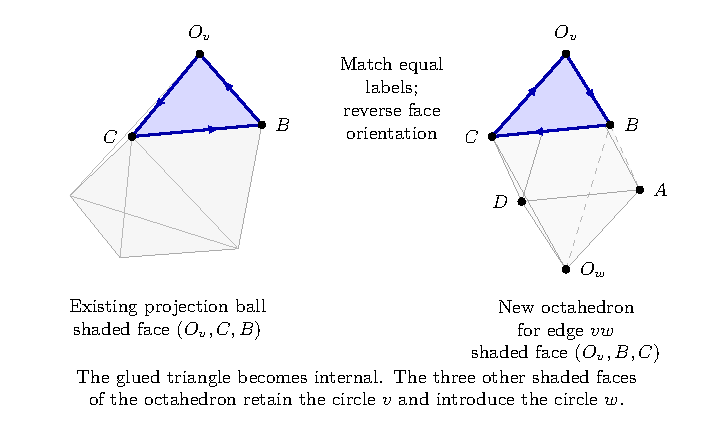
\includegraphics[width=.94\linewidth,keepaspectratio]{../book/figures/octahedral-page-attachment.pdf}
\caption{One ordered page attachment glues an edge block along a shaded triangle, retaining circle v and introducing circle w.}
\end{figure}

The attachment follows the original order of the tangle factors.
Its shaded triangle is glued to the designated disk page; the remaining
faces carry the new circle and the continuing main strands.

\subsection{Positive main meridians and their flags}\label{gi:positive-main-meridians-and-their-flags}

The bipartition signs describe native page coordinates. They are
not extra choices of the knot orientation. At a main boundary
vertex, take the actual small oriented meridian word supplied by
the physical collar. Its local derivative at the displayed ideal
point is \(m\) or \(m^{-1}\), depending on whether that native
meridian is the positive one or its inverse. Transport the word
and its eigenflag together through each face map.

For a main component, choose its orientation at one segment.
The same oriented small meridian propagates by the actual
annular collar conjugacies. The geometric ideal flag propagates
by those same conjugacies, so its chosen eigenvalue stays fixed.
There is no freedom to exchange it after returning around the
component: for generic \(M\), the peripheral longitude commutes
with a nonparabolic meridian and hence preserves both eigenlines.
At \(M=1\) use the analytic limit of this transported flag.
Thus one can record which global component orientation makes
the displayed flag the \(M^{-1}\) source flag. For a knot this
is one global orientation choice, not a separate reset at each
edge. A comparison with an already specified positive
meridian must make this initial choice explicitly.

This argument identifies the local auxiliary products for the
pure tree. Sections~\ref{gi:boundary-isotropy-and-the-edge-differential}--\ref{gi:determining-the-monomial-and-the-preferred-framing} identify the preferred main longitude
using the full boundary representation and its framing.

\subsection{Why the old odd three-point maps cannot be inserted unchanged}\label{gi:why-the-old-odd-three-point-maps-cannot-be-inserted-unchanged}

In the local chart keep the pure white maps \(W_j\) fixed.
Let \(A_{\mathrm o}\) and \(B_{\mathrm o}\) be the unique
three-point maps with the old odd permutations
\[
 (A,\infty,1)\mapsto(a,S,0),\qquad
 (A,R,0)\mapsto(a,\infty,1).
\]
They are

\begin{equation}\label{gi:S6}
A_{\mathrm o}=
 \begin{pmatrix}S&-S\\1&S(A-1)/a-A\end{pmatrix},\qquad
 B_{\mathrm o}=
 \begin{pmatrix}(a(A-R)+R)/A&-R\\1&-R\end{pmatrix}.
\end{equation}

The first original odd edge return is not trivial:

\begin{equation}\label{gi:S7}
W_0^{-1}B_{\mathrm o}W_2^{-1}A_{\mathrm o}:
             z\longmapsto m^{-2}z+(1-m^{-2})A.
\end{equation}

The second return is likewise nontrivial; the third,
\(W_1^{-1}B_{\mathrm o}W_3^{-1}A_{\mathrm o}\), is
projectively the identity. In particular the two defects vanish
at \(M=1\), which is why the old parabolic calculation did not
detect them.

Equation \eqref{gi:S7} is an obstruction to keeping both the pure white
charts and the old odd vertex assignment. It is not an
obstruction to the half-twist homeomorphism. That homeomorphism
must transport the puncture eigenflags and the adjacent charts.

\subsection{A regular matrix implementing the actual positive braid collar}\label{gi:a-regular-matrix-implementing-the-actual-positive-braid-collar}

Let \(a,b\in\mathrm{SL}_2(\mathbb C)\) be the two ordered
puncture meridians in the physical braid frame. They have the
same trace \(M+M^{-1}\). The original positive crossing
convention is

\begin{equation}\label{gi:S8}
(a,b)\longmapsto(a^{-1}ba,a),\qquad P=ba.
\end{equation}

This is the literal Wirtinger rule of
\href{https://sashakolpakov.github.io/murakamis_dream/notes/marked_braid_holonomy.html}{the marked braid calculation},
section 5. In particular the preserved product is \(ba\),
not \(ab\).

Put

\begin{equation}\label{gi:S9}
H=P^{-1}-I.
\end{equation}

Near the auxiliary complete lift \(P\), whose trace is \(-2\),
\(\det H=2-\operatorname{tr}P\) is near \(4\).
There is no singular diagonalizing frame.
The Cayley--Hamilton identities for \(a,b\), with their equal
traces, give

\begin{equation}\label{gi:S10}
(P-I)a=b(P-I),\qquad
 (P-I)^2=(\operatorname{tr}P-2)P.
\end{equation}

Consequently \(H\) is projectively \((P-I)^{-1}\), it
commutes with \(P\), and

\begin{equation}\label{gi:S11}
HaH^{-1}=a^{-1}ba,\qquad HbH^{-1}=a.
\end{equation}

This is the exact positive collar rule \eqref{gi:S8}. Its inverse realizes
the negative crossing.

Suppose the selected auxiliary flag has \(P\)-eigenvalue
\(-Q\). The eigenvalue ratio of \(H\) at that flag is

\begin{equation}\label{gi:S12}
\frac{-Q^{-1}-1}{-Q-1}=Q^{-1}.
\end{equation}

Thus composing a pure auxiliary meridian with \(H^\epsilon\)
changes its similarity by \(Q^{-\epsilon}\). It keeps the
disk longitude \(P\) and its chosen flag.

There is an independent matrix calibration against the original
geometric collar. In the local chart set

\begin{equation}\label{gi:S13}
P=m^{-1}W_2^{-1}W_0.
\end{equation}

This is the determinant-one disk word and has selected
eigenvalue \(-Q\). At \(m=1\), for all nearby \(E_0,Q\),
not just at the complete point,

\begin{equation}\label{gi:S14}
S_v^{-1}(P^{-1}-I)=W_0^{-1}B_{\mathrm o}
                        \quad\text{projectively}.
\end{equation}

The right side is the original physical positive-\(R\)
meridian, by section 6 of
\href{https://sashakolpakov.github.io/murakamis_dream/notes/actual_conway_general_mask_marked_filling.html}{the marked mask filling proof}.
Its inverse crossing is the other old odd path.
Equations \eqref{gi:S8} and \eqref{gi:S14} fix both the braid sign and the actual
copy/collar marking; the sign has not been chosen from a desired
source formula.

\subsection{The full ordered boundary groups in the actual edge chart}\label{gi:the-full-ordered-boundary-groups-in-the-actual-edge-chart}

Let \(N_j=W_{j-1}^{-1}W_j\), with indices modulo four.
Their determinant-one lifts, in the order of the original
equatorial boundary, are

\begin{equation}\label{gi:S14a}
A_g=M^{-3}N_3,\qquad B_g=MN_0,\qquad
 C_g=MN_1,\qquad D_g=MN_2,\qquad
                    A_gB_gC_gD_g=I.
\end{equation}

Each trace is \(M+M^{-1}\). These lifts follow from
\(\det W_0=L,\det W_1=L/m,\det W_2=L/m^2,\det W_3=Lm\).
They include the native loop directions, which need not all be
positive main meridians.

The pure edge returns give the following complete boundary
intertwinings:

\begin{equation}\label{gi:S14b}
\begin{array}{c|c|c|c|c}
 \text{circle}&(a,b)\text{ on the input side}
 &(a',b')\text{ on the output side}&C_0&P=ba=b'a'\\ \hline
 v&(B_g,A_g)&(C_g^{-1},D_g^{-1})&S_v^{-1}&A_gB_g\\
 w&(B_g^{-1},C_g^{-1})&(A_g,D_g)&S_w^{-1}&(B_gC_g)^{-1}.
\end{array}
\end{equation}

Here \(C_0aC_0^{-1}=a'\) and \(C_0bC_0^{-1}=b'\).
For example the first row is equivalent to

\begin{equation}\label{gi:S14c}
S_v C_g S_v^{-1}=B_g^{-1},\qquad
 S_v D_g S_v^{-1}=A_g^{-1}.
\end{equation}

The second is equivalently
\(S_w A_gS_w^{-1}=B_g^{-1}\) and
\(S_w D_gS_w^{-1}=C_g^{-1}\).
These are consequences of the full white/shaded returns;
they may also be checked by direct multiplication of the local
matrices. The product columns agree because
\(D_g^{-1}C_g^{-1}=A_gB_g\) and
\(D_gA_g=(B_gC_g)^{-1}\).

The disk convention \(P=ba\) is therefore explicit at both
ends, including the inversions caused by the turned second
circle. The same table transports under the actual conjugating
frames in a tree; an orientation reversal transports the whole
tuple and its disk word. It does not silently replace \(P\)
by a different boundary product.

For the positive braid put \(H=P^{-1}-I\) in the input
frame. Then \(C_+=C_0H\) satisfies

\begin{equation}\label{gi:S14d}
\begin{aligned}
 C_+aC_+^{-1}&=a'^{-1}b'a',\\
 C_+bC_+^{-1}&=a',\\
 C_+PC_+^{-1}&=P .
\end{aligned}
\end{equation}

For the negative braid use \(H^{-1}\) and the inverse
automorphism. Thus the construction checks both generators of
the actual twice-punctured disk and its outer boundary word;
it is stronger than checking a peripheral similarity or three
traces. Formula \eqref{gi:S14} fixes the positive crossing in the
original physical convention.

\subsection{The opposite-eigenflag qualification}\label{gi:the-opposite-eigenflag-qualification}

Let \(F_a,F_b\) be the two displayed puncture flags, with
eigenvalues \(\lambda_a,\lambda_b\). The natural braid output
flags for \eqref{gi:S8} are

\begin{equation}\label{gi:S15}
(a^{-1}F_b,F_a).
\end{equation}

Their eigenvalues are \((\lambda_b,\lambda_a)\), since
the strands have exchanged positions. By contrast,
\((HF_a,HF_b)\) has eigenvalues
\((\lambda_a,\lambda_b)\) on that same output tuple.
If the selected eigenvalues agree, the two descriptions coincide
by uniqueness of the relevant eigenline. If they differ, use
\(H\) on the opposite input eigenlines to obtain \eqref{gi:S15}.
At a native pure circle the geometric flags on its two main
punctures have opposite selections \(M^{-1},M\).
The qualification is therefore essential.

This identifies the error in an unqualified instruction to
transport both displayed flags by \(H\). The intertwiner is
correct; the displayed decorated triangle needs the accompanying
Weyl change. The two eigenlines coalesce at the parabolic point,
so the complete figure alone cannot distinguish the operations.

\subsection{Representation gluing followed by global decoration}\label{gi:representation-gluing-followed-by-global-decoration}

The following construction keeps that distinction explicit.
First perform the actual collar gluing at the level of
representations; then select the geometric eigenflags on the
resulting original link group.

The half-twist is the actual mapping cylinder of the two-punctured
disk, fixing its outer boundary. Its two boundary generator
tuples are related by \eqref{gi:S8}. If \(C\) is the pure boundary
intertwiner, replacing it by \(CH^\epsilon\), with the side
and composition order fixed by \eqref{gi:S14}, supplies the new
intertwiner. Equation \eqref{gi:S11} verifies the two puncture relations;
\([H,P]=0\) verifies the outer disk-boundary relation. These
are the generators and relation of the twice-punctured disk.
The van Kampen presentation of that actual cut therefore gives
the representation of the reglued exterior. It uses the one
distinguished disk seam at that circle, once.

Apply the operation in every original circle's transported
puncture frame. The other cyclic page seams remain those of
the pure-page construction above. At this stage no assertion is made that the old
pure ideal vertices still provide the correct decoration.

For each resulting main component, choose its actual positive
meridian and its \(M^{-1}\) eigenflag. At a corner whose
native loop is the inverse, take the corresponding \(M\)
eigenflag. Transport these choices by the original paths in the
completed cut. Peripheral commutation makes the choice independent
of a peripheral path. Keep the already selected disk-longitude
flag on each auxiliary circle.

These choices are holomorphic near the complete structure.
For example, for a noncentral matrix
\(\left(\begin{smallmatrix}a&b\\c&d\end{smallmatrix}\right)\)
with \(b\ne0\), an eigenline with prescribed holomorphic
eigenvalue \(\lambda\) is represented by
\((b,\lambda-a)\). The opposite eigenline is obtained by
replacing \(\lambda\) by \(\lambda^{-1}\).
Both approach the unique parabolic flag at the complete point.
A change of coordinate handles a chart with \(b=0\).
The same argument applies to the selected auxiliary eigenvalue
\(-Q\).

Develop the original topological ideal triangulation from these
global flags and the constructed representation. The map of
each triangle is the unique map of its transported ordered
triple. Adjacent white maps must be rebuilt in this way;
\eqref{gi:S7} shows why they cannot generally be retained unchanged.
Equivariance gives every edge return. At the complete parameter,
\eqref{gi:S14} and the original collar convention identify the actual odd
development. Its positively oriented tetrahedra therefore remain
positive in a sufficiently small neighborhood of the fixed
finite tree. This is a local decorated representation
construction, not a global completeness assertion for a
nonparabolic main cusp.

The tuple with \(P=ba\) is exactly \eqref{gi:S14b}, transported in the
original physical collar. The positive main loops are chosen
in the completed cut. For the canonical four-segment traversal,
they are \(C_g,B_g^{-1},A_g,D_g^{-1}\) at
\(\infty,0,R,1\), respectively; all four select their geometric
corner with eigenvalue \(M^{-1}\). A reversed physical route
transports both its loop direction and its flag. The preceding
opposite-eigenflag calculation describes the required Weyl change.

At representation level the primitive auxiliary increment is

\begin{equation}\label{gi:S16}
U_v^{\exp}
       =Q_v^{-\epsilon_v}
          \prod_{e\ni v}\frac{Q_v+X_e}{1+Q_vX_e},\qquad
 V_v^{\exp}=Q_v^2.
\end{equation}

It is unchanged by the main-flag redecoration. The exponentiated filling
equation with \(n_v=\epsilon_v-2p_v\) is then

\begin{equation}\label{gi:S17}
\prod_{e\ni v}\frac{Q_v+X_e}{1+Q_vX_e}
                                =Q_v^{n_v}.
\end{equation}

The auxiliary formulas retain the original circle words. The main
preferred longitude is determined in Sections~\ref{gi:boundary-isotropy-and-the-edge-differential}--\ref{gi:determining-the-monomial-and-the-preferred-framing} using boundary
isotropy, algebraic regularity and the independently marked cusp.
The argument does not replace a boundary word by a scalar simply
because the local representation has the correct traces.

\section{The complete anchor and the primitive filling equations}\label{gi:the-complete-anchor-and-the-primitive-filling-equations}

At \(M=1\), the local charts reduce to the
\href{https://sashakolpakov.github.io/murakamis_dream/notes/actual_all_circle_angular_octahedra.html}{angular octahedral charts}.
Their white/shaded words and primitive disk longitude agree with the
ones above. Their complete flags and oriented tetrahedral shapes
give the marked complete structure of the original augmented
exterior. The
\href{https://sashakolpakov.github.io/murakamis_dream/notes/general_marked_multicusp_gluing_rigidity.html}{multicusp gluing rigidity theorem}
identifies the nearby decorated representation with that marked
geometric germ; this uses the full original peripheral rows, not
only equality of their traces.

The pure meridian increments multiply around each circle in its
actual cyclic order. The one retained half twist contributes
\(Q_v^{-\epsilon_v}\), with the sign calibrated in \eqref{gi:S14}.
Thus, on the continued marking,

\begin{equation}\label{gi:A1}
U_v=\sum_{e\ni v}\log\rho_{v,e}-\epsilon_v\log Q_v,\qquad
 V_v=2\log Q_v.
\end{equation}

These are logarithms of the squared eigenvalues of the original
primitive auxiliary curves. No peripheral power is substituted.

For a branch supplied by the
\href{https://sashakolpakov.github.io/murakamis_dream/notes/actual_all_circle_geometric_completion.html}{geometric completion theorem}
or the corresponding marked long-filling theorem, the original
primitive logarithmic equation is

\begin{equation}\label{gi:A2}
U_v+p_vV_v=-2\pi i.
\end{equation}

Its continued mark selects the original first-charge geometric
branch. More explicitly, let \(\Psi(\tau)\) be the angular action
obtained after the original wire variables have been made stationary,
with \(Q_v=e^{i\tau_v}\). The marked circle calculation gives
\(U_v=-2\pi\Psi_{\tau_v}-i\epsilon_v\tau_v\).
The charge path is therefore exactly

\begin{equation}\label{gi:A2a}
\Psi_{\tau_v}+\frac{in_v\tau_v}{2\pi}-ic=0
 \quad\Longleftrightarrow\quad
 U_v+p_vV_v=-2\pi ic,\qquad 0\le c\le1.
\end{equation}

The logarithms are continued from the complete point at \(c=0\);
the constant \(-ic\) is part of the primitive mark.
Exponentiation at \(c=1\) gives \eqref{gi:T5}, since
\(n_v=\epsilon_v-2p_v\). The exponentiated equation alone
does not select the logarithmic branch or prove smooth completion.
At the selected filled point write \(Q_v=e^{i\tau_v}\).
The completion has \(\operatorname{Im}\tau_v<0\), hence
\(Q_v^2\ne1\). Its auxiliary longitude is therefore semisimple
with distinct eigenlines. The filling word commutes with that longitude;
equation \eqref{gi:T5} says that its eigenvalue ratio is one. A matrix commuting
with a matrix having distinct eigenlines is diagonal in that eigenbasis,
so ratio one makes it scalar. Thus the filling word is projectively
identity, and this conclusion persists on a sufficiently small
neighborhood of the selected filled point.

The marked charge path identifies the representation at \(M=1\),
not only its peripheral eigenvalues. It begins with the original
complete octahedral charts. Along the path the same labeled face maps,
primitive disk curves and source \(M^{-1}\) flag are retained.
The positive-cell completion identifies its endpoint with the
holonomy of the original complete filled knot. For the marked
long-filling branch the same identification follows from its original
Dehn-filling construction.

When the selected source critical point is nondegenerate, its
implicit branch gives holomorphic \(Q_v(M)\) and \(X_e(M)\) near
that endpoint, retaining \eqref{gi:A2}. The reconstructed matrices then give
a branch of representations of the original filled group by the
preceding semisimple argument. The geometric meridian coordinate
is a local parameter at complete knot holonomy, by the
\href{https://sashakolpakov.github.io/murakamis_dream/notes/actual_geometric_normal_period.html\#3-the-geometric-critical-scheme-is-smooth-with-two-framing-directions}{geometric knot-germ construction}
and its marked gluing input. The
\href{https://sashakolpakov.github.io/murakamis_dream/notes/general_marked_multicusp_gluing_rigidity.html}{multicusp version}
supplies the corresponding representation and decoration comparison
where a positive complete triangulation is specified.
Consequently this branch is the geometric meridian germ with the
declared eigenflag. This is the branch used when a source asymptotic
is later compared with the geometric longitude.

Every statement below about a filled geometric longitude retains
this original complete/filling anchor. An exponentiated slope equation
on a different algebraic branch is insufficient.

\section{Boundary isotropy and the edge differential}\label{gi:boundary-isotropy-and-the-edge-differential}

\subsection{The edge equation and a closed differential}\label{gi:the-edge-equation-and-a-closed-differential}

For an edge with endpoint variables \(Q,P\), let \(X\) satisfy

\begin{equation}\label{gi:R1}
(X+Q)(X+Q^{-1})(X+P)(X+P^{-1})
      =(X-1)^2(1-XM^2)(1-X/M^2).
\end{equation}

The variables are nonzero. We work first where all displayed factors
are nonzero and the selected root is simple. Write

\begin{equation}\label{gi:R2}
\begin{gathered}
 u=\log M,\quad q=\log Q,\quad p=\log P,\quad z=\log X,\\
 f=\frac{M^2-X}{1-M^2X},\quad
 \rho_Q=\frac{Q+X}{1+QX},\quad
 \rho_P=\frac{P+X}{1+PX}.
 \end{gathered}
\end{equation}

Only the differentials of the logarithms will be used. Their branches
therefore do not affect the identities below.

Let \(F\) be the logarithm of the quotient of the two sides of
\eqref{gi:R1}, holding \(z,q,p,u\) independent before differentiating.
Direct differentiation gives

\begin{equation}\label{gi:R3}
F_u=2(\log f)_z,\qquad
 F_q=-(\log\rho_Q)_z,\qquad
 F_p=-(\log\rho_P)_z.
\end{equation}

On the edge surface \(dF=0\). Moreover \(f\) has no direct
\(q,p\) dependence, and each \(\rho\) has no direct
\(u\) dependence or dependence on the other endpoint. Thus

\begin{equation}\label{gi:R4}
\begin{aligned}
 &du\wedge d\log f+
   \tfrac12d\log\rho_Q\wedge dq+
   \tfrac12d\log\rho_P\wedge dp\\
 &\quad=\tfrac12(F_u\,du+F_q\,dq+F_p\,dp)\wedge dz=0.
 \end{aligned}
\end{equation}

This proof uses the rational equation itself. It does not identify a
geometric volume by comparing numerical critical values. Since \eqref{gi:R4} is
an identity of rational differential forms, it holds on every smooth
part of the same algebraic component.

\subsection{The actual boundary pairing}\label{gi:the-actual-boundary-pairing}

Sections~\ref{gi:the-local-face-maps}--\ref{gi:ordered-pages-and-the-half-twist-collar} have assembled the ordered pieces into a representation
of the original augmented link exterior. Let \(L\) be the
eigenvalue of its preferred main longitude on the main
\(M\)-eigenline. At each auxiliary circle let \(U_v\) be the
logarithm of the primitive meridian similarity, and let the selected
longitude eigenvalue be \(-Q_v\). The exact local construction and
the original half-twist convention give

\begin{equation}\label{gi:R5}
U_v=\sum_{e\ni v}\log\rho_{v,e}-\epsilon_v\log Q_v,
 \qquad \epsilon_v\in\{-1,0,1\},
\end{equation}

up to locally constant logarithmic periods. The summands and the
primitive word must be established by the actual boundary gluing.

The infinitesimal boundary pairing is

\begin{equation}\label{gi:R6}
du\wedge d\log L+
             \tfrac12\sum_v dU_v\wedge d\log Q_v=0.
\end{equation}

Here all tori use the meridian--longitude orientations induced by the
same oriented exterior. The factor one half occurs because \(U_v\)
is a logarithm of an eigenvalue ratio, whereas \(\log Q_v\) is
a logarithm of a single determinant-one eigenvalue.

For completeness, \eqref{gi:R6} has a direct topological proof. Infinitesimal
variations of a representation are one-cocycles with values in its
adjoint local system. Pair two such cocycles by
\(\operatorname{tr}(XY)\) and take their cup product. The result
is a closed ordinary two-cochain, because the trace pairing is
invariant under conjugation. Its total evaluation on the boundary
of a fundamental three-chain is zero by the cochain Stokes identity.
On a torus with commuting diagonal holonomies, write their logarithms
as \(x\operatorname{diag}(1,-1)\) and
\(y\operatorname{diag}(1,-1)\). The alternating trace pairing
is \(2(dx\wedge dy)\). Summing over the boundary tori gives
\(\sum dx\wedge dy=0\). Substitute
\((x,y)=(u,\log L)\) at the main torus and
\((x,y)=(U_v/2,\log Q_v)\) at the auxiliary tori. This proves
\eqref{gi:R6} where the peripheral matrices are diagonalizable. The rational
identity extends over the remaining points where its terms are defined.

Subtract the sum of \eqref{gi:R4} over all edges from \eqref{gi:R6}. The half-twist term
in \eqref{gi:R5} has zero wedge product with \(d\log Q_v\). The result is

\begin{equation}\label{gi:R7}
du\wedge d\log\left(\frac{L}{\prod_e f_e}\right)=0.
\end{equation}

In particular, the discrepancy has no infinitesimal dependence on any
auxiliary variable. To avoid choosing determinant-one lifts globally,
use the squared discrepancy

\begin{equation}\label{gi:R8}
R=\frac{L^2}{\prod_e f_e^2}.
\end{equation}

It is a rational function whenever the original projective peripheral
representation is rational on the source variety: \(L^2\) is the
ratio of the two eigenvalues of the main longitude, with its ordered
main flag retained.

\section{The constant field of the source equations}\label{gi:the-constant-field-of-the-source-equations}

\subsection{Why the discrepancy is rational in the main meridian}\label{gi:why-the-discrepancy-is-rational-in-the-main-meridian}

Let \(k=\mathbb C(M)\), and let the graph have distinct unordered
edges. In particular this applies to a tree. The edge quadratic
gives, on putting \(Z=X+X^{-1}\):

\begin{equation}\label{gi:R9}
Z=\frac{2(M^2+M^{-2})-(Q+Q^{-1})(P+P^{-1})}
 {Q+Q^{-1}+P+P^{-1}+M^2+M^{-2}+2}.
\end{equation}

Work on the open set where these denominators are invertible; it
contains the complete branch. The squareclass of \(Z^2-4\) is

\begin{equation}\label{gi:R10}
H_e=(Q_v-1)^2(Q_w-1)^2
                  -4(M+M^{-1})^2Q_vQ_w.
\end{equation}

To see that the edge squareclasses are independent, extend the
coefficient field to an algebraic closure \(\overline{k}\).
Put \(t=(M+M^{-1})^2\ne0\) in this field. As a quadratic in
\(Y\), the polynomial
\((X-1)^2(Y-1)^2-4tXY\) has discriminant

\begin{equation}\label{gi:R11}
16tX[X^2+(t-2)X+1].
\end{equation}

Its order of vanishing at \(X=0\) is one, so it is not a square
in \(\overline{k}(X)\). Its coefficients in \(Y\) have no
common factor: at \(X=1\) the middle coefficient is \(-4t\).
It is therefore irreducible in \(\overline{k}[X,Y]\).

Different edges give different such prime polynomials, since they
involve different pairs of independent vertex variables. The valuation
at the prime \(H_e\) is odd for its own squareclass and zero for
every other edge. Hence every nonempty product of edge squareclasses
is nonsquare. Adjoining their square roots has degree \(2^{|\mathcal E|}\)
even after extending \(k\) to \(\overline{k}\). This proves
geometric integrality of the generic source fiber over \(M\).
In particular \(k\) is algebraically closed in its function
field \(\mathcal F\).

The logarithmic derivatives in all the \(Q_v\) extend uniquely
to the finite separable field \(\mathcal F\). If an element of
\(\mathcal F\) is killed by every such derivative, its relative
differential over \(k\) vanishes. In characteristic zero it is
algebraic over \(k\), and therefore belongs to \(k\) by the
preceding paragraph. Applying this to \eqref{gi:R7}--\eqref{gi:R8} gives

\begin{equation}\label{gi:R12}
R\in\mathbb C(M)^*.
\end{equation}

The specialization of \eqref{gi:R10} at \(M=\pm i\) is a square. This
does not invalidate the generic integrality proof; it does mean that
those fibers need the separate check in Section~\ref{gi:regular-reconstruction-at-every-nonzero-main-value}.

\section{Regular reconstruction at every nonzero main value}\label{gi:regular-reconstruction-at-every-nonzero-main-value}

\subsection{A uniform algebraic open set in every fiber}\label{gi:a-uniform-algebraic-open-set-in-every-fiber}

For one edge write

\begin{equation}\label{gi:G1}
m=M^2,\quad D=m+m^{-1},\quad
 \beta=Q+Q^{-1},\quad\gamma=P+P^{-1},\quad
 S=\beta+\gamma+D+2.
\end{equation}

Use \(X\) for the source wire coordinate. Its equation is the
quadratic

\begin{equation}\label{gi:G2}
F(X)=S(X^2+1)+(\beta\gamma-2D)X=0.
\end{equation}

This is equivalent, on \(X\ne0\), to the original degree-four
effective edge equation after its cancellation. Define

\begin{equation}\label{gi:G3}
J=\beta\gamma-2\beta-2\gamma-4D-4.
\end{equation}

The discriminant of \eqref{gi:G2} is

\begin{equation}\label{gi:G4}
\Delta=(\beta+2)(\gamma+2)J.
\end{equation}

Consider the open conditions

\begin{equation}\label{gi:G5}
\begin{gathered}
 QP\ne0,\qquad
 (\beta+2)(\gamma+2)(\beta+D)(\gamma+D)\ne0,\\
 S\ne0,\qquad \Delta\ne0.
\end{gathered}
\end{equation}

For every fixed \(M_0\in\mathbb C^*\), these conditions define
a nonempty Zariski open subset of the \(Q,P\) torus. Indeed each
excluded expression is a nonzero polynomial in the independent
variables \(\beta,\gamma\). For a fixed finite tree the same
conditions can be imposed simultaneously at every edge, since
their product is again a nonzero Laurent polynomial in the
vertex parameters \(Q_v\).

On \eqref{gi:G5}, both roots of \eqref{gi:G2} are finite, nonzero and distinct.
Several useful evaluations are

\begin{equation}\label{gi:G6}
\begin{aligned}
 F(1)&=(\beta+2)(\gamma+2),&
 F(-1)&=-J,\\
 F(m)&=m(\beta+D)(\gamma+D),&
 F(m^{-1})&=m^{-1}(\beta+D)(\gamma+D).
\end{aligned}
\end{equation}

Hence neither root is \(1,-1,m,m^{-1}\). In particular

\begin{equation}\label{gi:G7}
f=\frac{m-X}{1-mX}
\end{equation}

is a finite nonzero function at every point under consideration.
The auxiliary factors \((Q+X)/(1+QX)\) and
\((P+X)/(1+PX)\) are also finite and nonzero. To see this,
substitute \(X=-Q\) or \(X=-Q^{-1}\) in the original edge
equation. A zero can occur only when \(Q=-1\) or
\(Q=-m^{\pm1}\), excluded by \eqref{gi:G5}; the other endpoint is
identical.

\subsection{The actual character matrices remain regular}\label{gi:the-actual-character-matrices-remain-regular}

Put \(t=M+M^{-1}\), \(p=-\beta\), \(q=-\gamma\), and
\(\mathcal X=2+SX\). The character adapter uses

\begin{equation}\label{gi:G8}
A=\begin{pmatrix}M&1\\0&M^{-1}\end{pmatrix},\qquad
 B=\begin{pmatrix}M^{-1}&0\\p-2&M\end{pmatrix}.
\end{equation}

Its matrix \(C\) is given by

\begin{equation}\label{gi:G9}
\begin{gathered}
 h=M-M^{-1},\qquad
 c=\frac{M\mathcal X+M^{-1}q-2t}{D-p},\\
 d=\frac{q-M^2-1+hc}{p-2},\qquad
 e=\mathcal X-1-M^{-2}-hc,\qquad
 C=\begin{pmatrix}c&d\\e&t-c\end{pmatrix},\\
                         D_0=(ABC)^{-1}.
\end{gathered}
\end{equation}

The only denominators in \eqref{gi:G8}--\eqref{gi:G9}, besides powers of \(M\),
are \(p-2=-(\beta+2)\) and \(D-p=D+\beta\).
They are units on \eqref{gi:G5}. The four matrices have determinant one
and trace \(t\), with
\(\operatorname{tr}(AB)=-\beta\) and
\(\operatorname{tr}(BC)=-\gamma\), by \eqref{gi:G2}.
The formulas contain no division by \(M-M^{-1}\) or by \(t\).

The pure auxiliary transports are

\begin{equation}\label{gi:G10}
V=AB-\frac{1+X(\beta+1)}{1-X}I,\qquad
 T=BC+\frac{X+\gamma+1}{1-X}I.
\end{equation}

They satisfy the full puncture conjugacies, not just the trace
equations. Their determinants simplify on \eqref{gi:G2} to

\begin{equation}\label{gi:G11}
\det V=\frac{X(\beta+2)^2(\beta+D)}{S(X-1)^2},\qquad
 \det T=\frac{X(\gamma+2)^2(\gamma+D)}{S(X-1)^2}.
\end{equation}

For example the first determinant before reduction is
\[
 \frac{(\beta+2)(X^2+\beta X+1)}{(X-1)^2}.
\]
Equation \eqref{gi:G2} implies
\(X+X^{-1}+\beta=(\beta+2)(\beta+D)/S\), giving \eqref{gi:G11}.
The second computation is the same with \(\gamma\).
Thus both full transport matrices and their inverses are regular
on \eqref{gi:G5}, on either root of the source equation.

Every disk boundary pair is irreducible there. For the first
pair the standard direct trace calculation gives

\begin{equation}\label{gi:G12}
\operatorname{tr}[A,B]-2=(\beta+2)(\beta+D)\ne0.
\end{equation}

The second has the corresponding \(\gamma\) formula.
One can also derive \eqref{gi:G12} directly from the two matrices \eqref{gi:G8}.
For determinant-one two-generator representations this
nonzero expression excludes a common invariant line. In
particular neither generator is central.

The positive odd collar uses \(H=P_{\mathrm{disk}}^{-1}-I\)
with the original ordered disk product. Since
\(\operatorname{tr}P_{\mathrm{disk}}=-\beta\),

\begin{equation}\label{gi:G13}
\det H=2+\beta\ne0.
\end{equation}

The same holds at the other endpoint. The actual positive and
negative Hurwitz generators and all fixed powers remain
invertible. Thus odd seams introduce no exceptional fixed
value of \(M\).

\subsection{Sewing finitely many blocks uses a rational finite atlas}\label{gi:sewing-finitely-many-blocks-uses-a-rational-finite-atlas}

The ordered page construction glues two boundary pairs whose
matrices are explicit rational functions of the edge variables.
Their identification is the actual one in the native table;
where a loop is inverted or its order reversed, that operation
is included before asking for an intertwiner.

After those marked identifications, the two ordered boundary
pairs have the same three traces and are irreducible by \eqref{gi:G12}.
Their intertwiner is the solution line of

\begin{equation}\label{gi:G14}
G a=a'G,\qquad G b=b'G.
\end{equation}

The solution line is one-dimensional, and every nonzero solution
is invertible. Indeed a nontrivial kernel or image would be an
invariant line for one of the two irreducible pairs. Existence
can be proved without using ideal vertices. For an irreducible
pair the four matrices \(I,a,b,ab\) span
\(\operatorname{Mat}_2\). Their multiplication table is
determined by the common trace \(t\) and product trace \(p\):

\begin{equation}\label{gi:G14a}
a^2=ta-I,\quad b^2=tb-I,\quad
 ab+ba=t(a+b)+(p-t^2)I.
\end{equation}

The same table for the primed pair gives an isomorphism of
the two full matrix algebras, hence conjugation by an
invertible matrix. Equivalently put both pairs in the
explicit form \eqref{gi:G8}; irreducibility ensures that the two
selected generator flags are distinct and that the
off-diagonal entry used to normalize the frame is nonzero.
Either proof retains the ordered generators, not just the
individual conjugacy classes.

Equation \eqref{gi:G14} is a finite linear system with rational entries.
Choose a nonzero maximal minor and normalize one coordinate
on its one-dimensional kernel. This gives a rational
intertwiner regular in a neighborhood of that point.
No single choice of minor has to work at all parameters.
The finitely many choices form a rational atlas; the resulting
representation and peripheral eigenvalue ratios are independent
of the scalar normalization of an intertwiner.

Start with one edge block. The actual page insertion joins each
new block to the preceding union along one marked disk side.
Its attaching graph is a tree of blocks, so this inductively
constructs a representation of the entire page-cut object with
all matrices regular. The distinguished pure or odd seam at
each circle is then installed using \eqref{gi:G10}, \eqref{gi:G13}, and the two
full generator conjugacies of its actual mapping cylinder.
Those formulas preserve its outer disk product. Van Kampen
therefore gives the representation of the original augmented
exterior. No arbitrary pants permutation or commutativity of
tangles is used.

For any fixed finite tree, intersecting the finitely many
necessary open charts gives a nonempty open set over the
fixed \(M_0\). Equivalently, at any good point one may choose
each nonzero intertwiner minor in succession, obtaining a
regular neighborhood of that point. This proves existence of
the required actual rational \(\mathrm{PGL}_2\) reconstruction
at every nonzero main parameter.

This step requires the actual marked boundary conjugacies,
not just a formal family of characters. They were identified
with the original cut in the page/collar proof and remain
rational identities on the present open sets.

\subsection{The exceptional-looking main parameters}\label{gi:the-exceptional-looking-main-parameters}

At \(M=\pm1\), one has \(D=2\). Conditions \eqref{gi:G5} simply
exclude \(\beta=-2,\gamma=-2\), together with the stated
nonzero discriminant and denominator. The main matrix in
\eqref{gi:G8} is a noncentral parabolic. Nothing in \eqref{gi:G8}--\eqref{gi:G14} divides
by its eigenvalue difference, so the reconstruction is regular.

At \(M=\pm i\), one has \(D=-2\). The source discriminant
becomes

\begin{equation}\label{gi:G15}
\Delta=(\beta^2-4)(\gamma^2-4).
\end{equation}

With \(\beta=Q+Q^{-1}\) and \(\gamma=P+P^{-1}\),
this is a square in \(\mathbb C(Q,P)\). The fiber therefore
splits; generic-fiber irreducibility must not be asserted
at these two values. Nevertheless \eqref{gi:G5} gives two distinct
simple roots at generic \(Q,P\), and all matrices \eqref{gi:G8}--\eqref{gi:G14}
are regular. The main punctures are semisimple, with
eigenvalues \(i,-i\) or \(-i,i\), and remain noncentral.
The two roots can be written explicitly as

\begin{equation}\label{gi:G15a}
X=-\frac{Q+P}{1+QP},\qquad
             X=-\frac{1+QP}{Q+P}.
\end{equation}

For generic \(Q,P\) they differ and avoid \(1,-1\).
Fixing these auxiliary values, the implicit-function theorem
for \eqref{gi:G2} therefore continues either root holomorphically in
\(M\) through \(M_0=i\) or \(-i\).

The native ideal cell chart explains a possible false alarm.
At \(m=-1\), its preliminary white coordinate \(E_0\)
satisfies

\begin{equation}\label{gi:G16}
(E_0P-E_0Q-PQ+1)(E_0PQ-E_0-P+Q)=0.
\end{equation}

On one branch the two minus-copy circle apices coincide; on
the other the plus-copy apices coincide. Thus that particular
eight-tetrahedron ideal subdivision degenerates. This does
not make the actual group matrices singular: \eqref{gi:G8}--\eqref{gi:G14} are
an explicit regular reconstruction at precisely those points.
The rigidity argument needs the latter, not a positive
triangulation at every complex value of \(M\).

\subsection{A regular nonzero main eigenvalue ratio}\label{gi:a-regular-nonzero-main-eigenvalue-ratio}

Every main peripheral word is a fixed finite product of the
regular invertible group matrices just constructed. Hence its
matrix and inverse are regular at the chosen point.
The main meridian is noncentral.

There is one important trace-zero detail. Commutation in
\(\mathrm{PGL}_2\) alone would allow a longitude to
exchange the two eigenlines of a trace-zero meridian.
Use the matrices on the local section through nearby \(M\).
Normalize the meridian \(\mu\) to determinant one.
Its projective commutation with a regular invertible
longitude representative \(L\) gives
\(L\mu L^{-1}=\kappa\mu\), where
\(\kappa^2=1\) by determinants. At the nearby parameters
with \(M+M^{-1}\ne0\), taking traces gives \(\kappa=1\).
Consequently the exact matrix identity

\begin{equation}\label{gi:G16a}
L\mu=\mu L.
\end{equation}

extends to the trace-zero point. The undesired
anticommuting component is not part of this continued
representation. This also follows as a rational identity
on the integral generic source family.

At \(M_0\ne\pm1\), choose
its specified eigenline locally; its eigenvalue on a commuting
peripheral word is finite and nonzero. The ratio of the two
peripheral eigenvalues is therefore a regular unit.

The same conclusion holds at \(M_0=\pm1\), without
diagonalizing the meridian. In a frame in which its
upper-right entry is a unit, a commuting matrix \(L\) has
the form

\begin{equation}\label{gi:G17}
L=aI+b\mu.
\end{equation}

Here \(b=L_{12}/\mu_{12}\) and
\(a=L_{11}-b\mu_{11}\) are regular. Its two selected
eigenvalues are \(a+bM\) and \(a+bM^{-1}\). Both are
nonzero at the point because \(\det L\ne0\).
Their ratio is therefore regular and nonzero through the
parabolic value. Scalar changes of the representative \(L\)
cancel from the ratio.

The selected meridian eigenline itself is regular as well:
in this frame it is spanned by
\((\mu_{12},M-\mu_{11})\), or by
\((\mu_{12},M^{-1}-\mu_{11})\) for the other selection.
The first coordinate is a unit, including at \(M=\pm1\).
Thus coalescence of the two flags does not create a pole in
the marked eigenvalue ratio.

This directly applies to the square of a determinant-one
preferred-longitude eigenvalue, with the chosen inverse
convention if necessary. It does not require choosing a
global square root of a projective matrix determinant.
Every factor \eqref{gi:G7}, and every framing monomial in \(M\),
is likewise a unit at the point.

\subsection{Local sections and the integral total family}\label{gi:local-sections-and-the-integral-total-family}

More concretely, fix generic numerical auxiliary values
\(Q_v=q_v\) satisfying all the open conditions at \(M_0\),
and choose a simple root of every edge equation. The implicit
function theorem gives simultaneous holomorphic roots
\(X_e(M)\) near \(M_0\). At the chosen point select a
nonzero minor in each linear gluing system \eqref{gi:G14}. Those same
minors remain nonzero nearby. All actual group matrices,
their inverses and the main eigenvalue ratio are then
holomorphic along this local section. This is stronger than
the existence of an isolated good point in a special fiber.

The split trace-zero fibers do not invalidate this argument.
Let \(B\) be the Laurent coordinate ring in \(M,Q_v\),
localized at all \(S_e\). Dividing \eqref{gi:G2} by \(S_e\) makes
every edge polynomial monic with constant term one. The
simultaneous source algebra is therefore free over \(B\),
with basis the products \(\prod_e X_e^{\epsilon_e}\),
\(\epsilon_e\in\{0,1\}\). The independent generic edge
squareclasses imply that its generic localization is a
single field of degree \(2^{|\mathcal E|}\). Freeness embeds the
source algebra into that field; in particular the total
source variety is integral and has no additional vertical
component. Its simple points at \(M=\pm i\) belong to
the closure of the same generic family. A rational identity
proved there therefore holds on the regular local section
just constructed.

\section{Determining the monomial and the preferred framing}\label{gi:determining-the-monomial-and-the-preferred-framing}

By Section~\ref{gi:the-constant-field-of-the-source-equations} the discrepancy is a rational function of \(M\).
By Section~\ref{gi:regular-reconstruction-at-every-nonzero-main-value} its pullback is a regular unit along a local section
through every \(M_0\ne0\). If it had a zero or pole at \(M_0\),
that nonzero order would persist on the section. Therefore it has
no zero or pole on \(\mathbb C^*\), and

\begin{equation}\label{gi:F1}
\frac{L_{\mathrm{aug}}^2}{\prod_e f_e^2}=cM^k,\qquad
                  c\ne0,\quad k\in\mathbb Z.
\end{equation}

This is the elementary classification of units of
\(\mathbb C[M,M^{-1}]\). At the complete main cusp every
\(f_e=1\) and \(L_{\mathrm{aug}}^2=1\), so \(c=1\).

The \href{https://sashakolpakov.github.io/murakamis_dream/notes/actual_all_circle_preferred_cusp.html}{preferred-cusp calculation}
is a marked face-word calculation on the same original exterior:

\begin{equation}\label{gi:F2}
\tau_{\mathrm{main}}
      =a_{\mathrm{aug}}+2i\sum_e\cot(\pi x_e),\qquad
 X_e=e^{2\pi ix_e},\qquad
 a_{\mathrm{aug}}=-w_\epsilon-\sum_v\epsilon_v.
\end{equation}

The integer includes the retained half twists and the preferred
zero-linking correction. It is not inferred from \eqref{gi:F1}.

For completeness, the cusp shape equals the logarithmic slope
of this geometric eigenvalue curve. Near a noncentral parabolic
meridian write a commuting determinant-one longitude as
\(aI+b\mu\). Its eigenvalues are \(a+bM^{\pm1}\).
At \(M=1\), its projective translation divided by the
meridian translation is \(b/(a+b)\). Differentiating the
determinant-one relation shows that
\(d\log L/d\log M\) has the same value. Thus \eqref{gi:F2}
computes this derivative with the specified marking.

Since \(f_e(1,X)=1\) for every \(X\), its first
derivative receives no contribution from the derivative
of the wire:

\begin{equation}\label{gi:F3}
\left.\frac{d\log f_e}{d\log M}\right|_{M=1}
       =2\frac{1+X_e}{1-X_e}
       =2i\cot(\pi x_e).
\end{equation}

Equations \eqref{gi:F1}--\eqref{gi:F3} give \(k=2a_{\mathrm{aug}}\), proving
\eqref{gi:T4}. Tangent agreement fixes the exponent only after the
preceding argument has excluded every other rational factor.

Now let \(\ell_v=\operatorname{lk}(K,C_v)\).
The crossing disk has exactly two main punctures, so
\(\ell_v=0\) for opposite local strand directions and
\(\ell_v=\pm2\) for parallel directions. In the augmented
exterior,

\begin{equation}\label{gi:F4}
[\lambda_{\mathrm{aug}}]=\sum_v\ell_v[\mu_v],
             \qquad [\lambda_v]=\ell_v[\mu_K].
\end{equation}

After filling \(\mu_v+p_v\lambda_v\), its meridian has
class \(-p_v\ell_v[\mu_K]\). The original main-boundary
word that becomes the preferred filled longitude is therefore

\begin{equation}\label{gi:F5}
\lambda_{\mathrm{fill}}
       =\lambda_{\mathrm{aug}}\,
                       \mu_K^{\sum_vp_v\ell_v^2}.
\end{equation}

This is a primitive integral basis change on the same main
torus. It is not an assertion that the augmented longitude
was already zero linking after surgery.

\begin{figure}
\centering
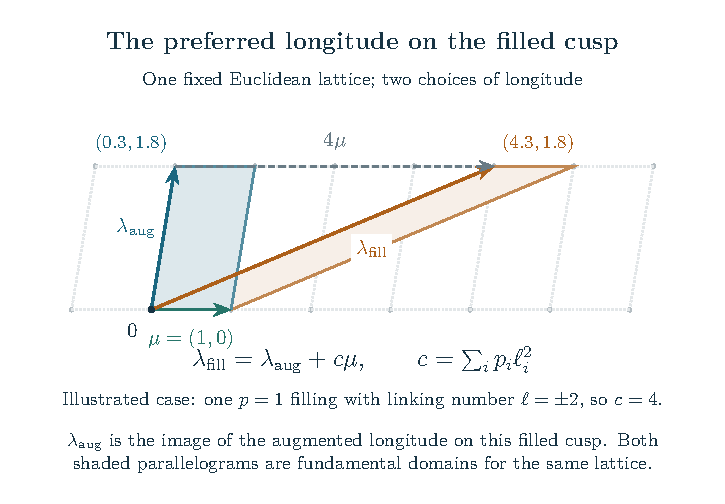
\includegraphics[width=.94\linewidth,keepaspectratio]{../book/figures/main-cusp-longitude-shear.pdf}
\caption{The image of the augmented longitude and the preferred filled longitude differ by an integral meridian shear on the same filled cusp.}
\end{figure}

Here \(\lambda_{\mathrm{aug}}\) means its image on the filled
cusp. Both shaded parallelograms use the same meridian and the
same lattice; the displayed example has
\(\sum_vp_v\ell_v^2=4\).

Write \(o_v=1\) for parallel and \(o_v=-1\) for
opposite strand directions in the fixed physical convention.
Then
\[
 \ell_v^2=2(1+o_v),\qquad
 w_\epsilon=\sum_vo_v\epsilon_v,\qquad
 w(D)=w_\epsilon-2\sum_vo_vp_v.
\]
Consequently

\begin{equation}\label{gi:F6}
\begin{aligned}
 a_{\mathrm{aug}}+\sum_vp_v\ell_v^2
  &=-w_\epsilon-\sum_v\epsilon_v+2\sum_vp_v(1+o_v)\\
  &=-w(D)-\sum_v(\epsilon_v-2p_v)=a(D).
\end{aligned}
\end{equation}

Combining \eqref{gi:T4} with \eqref{gi:F5}--\eqref{gi:F6} proves the squared filled
identity \eqref{gi:T6}, with the original primitive slopes and
preferred longitude.

\section{The determinant-one sign at the complete filled knot}\label{gi:the-determinant-one-sign-at-the-complete-filled-knot}

The squared identity leaves a two-valued ambiguity. Its sign is
fixed at the actual complete filled knot, rather than chosen
to fit the edge product.

The negative trace of a null-homologous peripheral curve is a known
fact; see Menal-Ferrer and Porti,
\cite[Corollary 3.10]{MenalFerrerPorti2012}.
The frame proof below includes the sign and its compatibility with
the lifts used here.

\subsection{A frame calculation on a once-bordered surface}\label{gi:a-frame-calculation-on-a-once-bordered-surface}

Let \(S\) be a compact connected oriented surface of genus \(g\)
with one boundary component. Embed it in an oriented three-manifold
which has a spin structure. Choose a smooth oriented tangent frame
\((e_1,e_2)\) on \(S\), and complete it by the positive unit normal
\(\nu\). Such a tangent frame exists because a surface with
boundary has trivial tangent bundle.

Pulling back the ambient spin double cover along
\((e_1,e_2,\nu)\) gives a double cover of \(S\).
Its monodromy is a homomorphism
\(H_1(S;\mathbb Z/2)\to\mathbb Z/2\).
Since the single oriented boundary is zero in this homology,
the lift of this chosen frame closes after one boundary circuit.

Now replace the first tangent vector on the boundary by its positive
unit tangent \(t\), and the second by the corresponding inward
tangent normal \(n\). Relative to \((e_1,e_2)\), the
frame \((t,n)\) has winding number

\begin{equation}\label{gi:L1}
\chi(S)=1-2g.
\end{equation}

This is the boundary form of the index formula: extend the outward
boundary normal to a tangent vector field with isolated zeros.
The sum of its indices is \(\chi(S)\); measured in the
global tangent frame, it is the degree of its boundary direction.
The boundary tangent differs from that normal by a fixed quarter
turn, which does not change the degree.

A full \(2\pi\) rotation in the tangent plane is the nontrivial
loop of the oriented three-dimensional frame group. It therefore
changes the sign of a spin lift. Formula \eqref{gi:L1} is odd. It follows
that the boundary-adapted frame

\begin{equation}\label{gi:L2}
(t,n,\nu)
\end{equation}

has an antiperiodic lift: after one boundary circuit its lift
returns to the other sheet.

No choice of spin structure changes this conclusion. The only
possible change was the monodromy of the first global frame,
and that monodromy vanishes on the boundary.

\subsection{Application to a complete hyperbolic knot cusp}\label{gi:application-to-a-complete-hyperbolic-knot-cusp}

Let \(Y\) be the oriented complete finite-volume hyperbolic complement
of a knot in \(S^3\). Take a sufficiently far cusp torus \(T\).
Its preferred longitude \(\lambda\) is primitive and bounds
a Seifert surface in the truncated complement.
Arrange the boundary of the surface to be the straight Euclidean
representative of \(\lambda\) on \(T\), and arrange its
collar to meet \(T\) orthogonally. These changes are made
inside the ordinary product collar of the boundary torus.

Along that boundary, \eqref{gi:L2} is a translation-invariant horospherical frame, up to
one constant rotation: \(t\) is the constant longitude
direction, \(n\) is the radial direction, and \(\nu\)
is the constant perpendicular direction in the horosphere.
Thus the preceding surface calculation says that the translation-invariant horospherical frame has
antiperiodic spin holonomy along \(\lambda\).

For precision, identify the oriented frame bundle of hyperbolic
three-space with \(\mathrm{PSL}_2(\mathbb C)\), and its
spin cover with \(\mathrm{SL}_2(\mathbb C)\).
Conjugate the cusp fixed point to infinity. If the longitude
translation is \(z_\lambda\ne0\), the path of translation-invariant
horospherical frames is represented by

\begin{equation}\label{gi:L3}
U(t)=
 \begin{pmatrix}1&t z_\lambda\\0&1\end{pmatrix},
                         \qquad 0\le t\le1.
\end{equation}

This is the lift starting at the identity.
Here translation-invariant refers to the cusp's Euclidean translation
group; no assertion of Levi-Civita parallel transport along a
horocycle in hyperbolic three-space is needed.
For a determinant-one holonomy lift \(\widetilde\rho\),
the endpoint of \eqref{gi:L3} closes in the quotient spin bundle precisely
when
\(\widetilde\rho(\lambda)=U(1)\).
It returns to the opposite sheet precisely when
\(\widetilde\rho(\lambda)=-U(1)\).
The antiperiodicity just proved therefore gives

\begin{equation}\label{gi:L4}
\boxed{\displaystyle
 \widetilde\rho(\lambda)=
       -\begin{pmatrix}1&z_\lambda\\0&1\end{pmatrix},
 \qquad
 \operatorname{tr}\widetilde\rho(\lambda)=-2.}
\end{equation}

Reversing the longitude replaces this matrix by its inverse and
does not change the sign. Any two determinant-one lifts differ
by a character to \(\{\pm1\}\), and the preferred longitude
is zero in the knot complement's first homology, so \eqref{gi:L4} is
independent of that choice as well.

Here spin existence needs no general three-manifold theorem.
Remove a point of the knot from \(S^3\); its complement is
\(\mathbb R^3\), whose standard tangent frame restricts to \(Y\).
Orthonormalizing for the hyperbolic metric gives a spin structure
on its oriented frame bundle and hence a lift of its geometric
holonomy. The sign calculation itself is the explicit surface-frame
argument above.

\subsection{Compatibility with the original augmented representation}\label{gi:compatibility-with-the-original-augmented-representation}

Return to the original all-circle construction. Write
\(\mu_K\) for its main meridian and \(\mu_v\) for its
original auxiliary meridians. The original circles are pairwise
unlinked. If \(\ell_v\) is the linking number of circle
\(v\) with the main knot and \(p_v\) is its integral
filling coefficient, the fixed main-boundary word which becomes
the preferred filled longitude is

\begin{equation}\label{gi:L5}
\lambda_{\mathrm{fill}}
       =\lambda_K\mu_K^{\sum_vp_v\ell_v^2}.
\end{equation}

In the augmented exterior its first homology class is

\begin{equation}\label{gi:L6}
[\lambda_{\mathrm{fill}}]
      =\sum_v\ell_v[\mu_v]
           +\sum_vp_v\ell_v^2[\mu_K].
\end{equation}

The original crossing disk is punctured by exactly two main
strands, so

\begin{equation}\label{gi:L7}
\ell_v\in\{0,2,-2\}.
\end{equation}

Consequently \eqref{gi:L6} vanishes modulo two.

At an actual complete filled knot point, pull back any
determinant-one lift of its complete holonomy to the augmented
group. Locally this lift continues through the augmented geometric
family: lift the finitely many generator matrices holomorphically;
the signs of the finitely many relations are discrete and remain
their identity values at the initial point.
If another local determinant-one lift is used for the face
construction, its ratio with this lift is a
\(\{\pm1\}\)-valued character: both project to the same
projective representation after one fixed conjugation.
By \eqref{gi:L6}--\eqref{gi:L7}, that character is one on
\(\lambda_{\mathrm{fill}}\).
Thus any such local face-map lift has exactly the same longitude
sign as the filled lift in \eqref{gi:L4}. A globally rational
determinant-one lift over the entire source variety is not
assumed or needed.

This step is useful because the original matrices of an auxiliary
filling slope may be \(-I\) rather than \(I\). One need not
assume that the particular auxiliary lifts descend to the filled
group. Their possible discrepancy is a character and cannot
change \eqref{gi:L5}.

\subsection{Fixing a holomorphic squared longitude identity}\label{gi:fixing-a-holomorphic-squared-longitude-identity}

The squared identity proved above, on a connected geometric germ
with the original selected main flag and fixed filling equations, is

\begin{equation}\label{gi:L8}
L_{\mathrm{geom}}^2
     =M^{2a(D)}
          \prod_e\left(\frac{M^2-X_e}{1-M^2X_e}\right)^2.
\end{equation}

The factors are holomorphic units near its complete filled point. Define
the longitude coordinate as the inverse eigenvalue on the source
\(M^{-1}\) meridian line. The ratio of the two sides before
squaring is then a holomorphic function taking values in
\(\{1,-1\}\); it is constant on the connected germ.

At the actual complete filled point, \(M=1\).
Each edge factor in \eqref{gi:L8} is one, since the geometric wire does
not have \(X_e=1\). The inverse selected longitude eigenvalue
is \(-1\) by the preceding complete-cusp and lift comparison. Therefore the constant is negative:

\begin{equation}\label{gi:L9}
\boxed{\displaystyle
 L_{\mathrm{geom}}
       =-M^{a(D)}
          \prod_e\frac{M^2-X_e}{1-M^2X_e}.}
\end{equation}

The conclusion requires the exact squared identity as input.
The complete-value sign fixes only its remaining two-valued
ambiguity; it is not being used to infer the dependence on \(M\)
or on any auxiliary parameter.

\section{The geometric factor of an actual quantum recurrence}\label{gi:the-geometric-factor-of-an-actual-quantum-recurrence}

The geometric identity now applies to the classical characteristic
selected by the actual invariant. This step uses the separate
\href{https://sashakolpakov.github.io/murakamis_dream/notes/actual_main_meridian_filtered_characteristic.html}{all-order source theorem};
the geometric construction by itself does not imply a quantum
asymptotic estimate.

\subsection{The source hypotheses and the factor statement}\label{gi:the-source-hypotheses-and-the-factor-statement}

Keep the original all-circle tree and knot qualifications of Section~\ref{gi:the-diagram-and-the-longitude-identity}.
Fix the signed powers and the diagram before the level tends to
infinity, and assume one of the following proved source hypotheses:

\begin{itemize}

\item
  the original strict presentation has independently sufficiently long
  fixed signed filling powers, as in the
  \href{https://sashakolpakov.github.io/murakamis_dream/notes/actual_main_meridian_filled_volume.html}{filled-meridian theorem};
\item
  its degrees and powers satisfy the
  \href{https://sashakolpakov.github.io/murakamis_dream/notes/actual_all_circle_quantitative_volume.html}{summed criterion},
  \(\sum_v d_v/(d_v^2+n_v^2)\le2^{-25}\);
\item
  they satisfy the
  \href{https://sashakolpakov.github.io/murakamis_dream/notes/actual_all_circle_local_message_volume.html}{local criterion},
  \(\max_v d_v/(d_v^2+n_v^2)\le2^{-120}\).
\end{itemize}

Here \(d_v\) is the number of edges incident to vertex \(v\).
The last two alternatives do not require every \(n_v\ne0\).
All original knot-pattern qualifications remain; in particular the
two-circle knot case excludes the two-odd link pattern. Both level
parities are retained.

Let \(F_N(M)\) be the actual zero-framed reduced ADO state, with

\begin{equation}\label{gi:O1}
q_N=e^{\pi i/N},\qquad M=-q_Nx,\qquad F_N(1)=K_N.
\end{equation}

The letter \(x\) here is the raw highest-weight parameter, not the
normalized internal index \(x_e\) with \(X_e=e^{2\pi ix_e}\).
Thus the marked complete meridian is \(M=1\). The
\href{https://sashakolpakov.github.io/murakamis_dream/notes/kashaev_ado_pointing.html}{ADO normalization and pointing} fix the
state and its complete value \(K_N\).

Consider any specified nonzero fixed operator

\begin{equation}\label{gi:O2}
P(q,M,T)=\sum_{j=0}^{d}a_j(q,M)T^j,\qquad
 a_j\in\mathbb C(q,M),\qquad TM=qMT,
\end{equation}

which annihilates the whole function \(F_N(M)\) at every sufficiently
large level \(q=q_N\). The shift \(T\) replaces \(M\) by \(qM\).
This is an actual all-level annihilator. Its existence is proved
independently by the
\href{https://sashakolpakov.github.io/murakamis_dream/notes/finite_sum_annihilator.html}{finite-sum annihilator theorem};
it is not defined by fitting complete values or by adding a desired
geometric factor.

Clear its fixed rational denominators to obtain Laurent-polynomial
coefficients, and remove their common \(q-1\) valuation. Let
\(P_0(M,L)\ne0\) be the first classical symbol that remains. If the
original operator has negative shift powers, first multiply by a
power of \(T\); this contributes only a Laurent unit to its
classical symbol.

Let \(A_{\mathrm{geom},\mathbb C}(M,L)\) generate the Laurent
prime of the actual oriented geometric eigenvalue germ through
\((M,L)=(1,-1)\). The longitude is the preferred one in \eqref{gi:T7},
on the \(M\) line, equivalently the inverse eigenvalue on the
source \(M^{-1}\) line.

\textbf{Corollary.} Under the stated all-circle source hypotheses,

\begin{equation}\label{gi:O3}
A_{\mathrm{geom},\mathbb C}(M,L)\mid P_0(M,L)
       \quad\text{in }\mathbb C[M^{\pm1},L^{\pm1}].
\end{equation}

This is the selected irreducible geometric factor, defined up to a
nonzero Laurent monomial. It is not a claim about its multiplicity,
the other factors of the symbol, or the full classical A-polynomial.
The rational-coefficient version is stated in Section~\ref{gi:the-irreducible-factor-and-its-field-of-definition}.

\subsection{The exact reduced/full conversion}\label{gi:the-exact-reducedfull-conversion}

The normalization factors must be retained before taking the
classical symbol. Write

\begin{equation}\label{gi:O4}
H_N(s)=\frac{\sin\pi s}{N\sin(\pi s/N)},\qquad
 d_N(M)=\eta_N\frac{M-M^{-1}}{M^N-M^{-N}},\qquad
 d_N(1)=\frac{\eta_N}{N},\quad \eta_N=i^{N+3}.
\end{equation}

The full modified-trace state is \(d_N(M)F_N(M)\). On
\(M=q_N^s\), the exact identity

\begin{equation}\label{gi:O5}
\frac{d_N(q_N^s)}{d_N(1)}=H_N(s)^{-1}
\end{equation}

shows that
\(\mathcal Z_N(s)=F_N(q_N^s)/(K_NH_N(s))\) is its normalized
full value. The source theorem makes \(K_N\ne0\) at every
sufficiently large level.

Put \(f(M)=M-M^{-1}\), distinct from the edge factors \(f_e\).
For every integer shift used in \eqref{gi:O2},

\begin{equation}\label{gi:O6}
\frac{d_N(q_N^jM)}{d_N(M)}
        =(-1)^j\frac{f(q_N^jM)}{f(M)}.
\end{equation}

The normalized full state therefore satisfies the root equation
of the fixed rational Ore operator

\begin{equation}\label{gi:O7}
\widetilde P=
   \sum_{j=0}^{d}a_j(q,M)(-1)^j
                        \frac{f(M)}{f(q^jM)}T^j.
\end{equation}

Multiplying on the left by \(\prod_{j=1}^{d}f(q^jM)\)
clears these additional denominators. After the same common
\(q-1\) valuation has been removed, its first classical symbol is

\begin{equation}\label{gi:O8}
f(M)^dP_0(M,-L).
\end{equation}

The meridian divisor and the sign character have both been
recorded. Neither is deleted by redefining the state.

\subsection{All orders, shifted charts and the geometric branch}\label{gi:all-orders-shifted-charts-and-the-geometric-branch}

The all-order source theorem proves, for every prescribed finite
order, an expansion

\begin{equation}\label{gi:O9}
\log\mathcal Z_N(s)\sim
       \sum_{r\ge1}N^{-r}p_r(s),\qquad \deg p_r\le r+1.
\end{equation}

Its proof uses the exact finite source on translated microscopic
charts, not analytic continuation of an asymptotic formula initially
known only on \(|s|<1\). For a fixed operator order \(d\), choose
a small open disk in the upper half-plane and retain all its
translates by \(0,1,\ldots,d\). Those compacts avoid ordinary-color
resonances. The same all-order expansion, with its original
normalization, holds at every shifted argument required by \eqref{gi:O7}.
If lower amplitudes depend on level parity, the argument is made
on either parity subsequence; the leading action is the same.

The degree bound in \eqref{gi:O9} is supplied by the canonical sine-factorial
interpolation and the original joint first-charge saddle. More
precisely, let \(\Phi\) be that joint phase at \(s=0\), including
the linear angular terms in \eqref{gi:A2a}. With its continued logarithms,
put

\begin{equation}\label{gi:O10}
\begin{aligned}
 J'(x)&=\log(2\sin\pi x),\\
 \mathcal K(x,t)&=2J(x)-J(x+t)-J(x-t),\\
 \Phi_t&=\Phi+\sum_{e\in\mathcal E}\mathcal K(x_e,t)
                       +\frac{\pi i\,a(D)}2t^2,\qquad
 S(t)=\Phi_t\bigl(\text{its selected critical point}\bigr).
 \end{aligned}
\end{equation}

The original Hessian is invertible, so the selected critical point
and \(S(t)\) are analytic near zero. The exact scalar in \eqref{gi:O10}
is the original zero-framing factor; no extra geometric phase has
been inserted.

The full stationary expansion has the form

\begin{equation}\label{gi:O11}
\log\mathcal Z_N(s)\sim
  N\{S(t)-S(0)\}
       +\sum_{j\ge0}N^{-j}\{C_j(t)-C_j(0)\},
          \qquad t=s/N,
\end{equation}

with holomorphic coefficient germs \(C_j\). Consequently the
coefficient of \(s^{r+1}\) in \(p_r(s)\) is exactly the coefficient
of \(t^{r+1}\) in \(S(t)-S(0)\); lower amplitudes cannot contribute
to that degree. This is the filtration needed for the operator
argument. A leading profile or finitely many microscopic jets
would not supply it.

Set \(h=\log q\), \(u=\log M=hs\), and define

\begin{equation}\label{gi:O12}
\mathcal S(u)=\pi i\{S(u/(\pi i))-S(0)\}.
\end{equation}

Regrading \eqref{gi:O9} by \(h^rs^k=h^{r-k}u^k\) gives

\begin{equation}\label{gi:O13}
h^{-1}\mathcal S(u)+\sum_{j\ge0}h^jA_j(u).
\end{equation}

The degree bound permits only the displayed negative power of
\(h\). Under the \(j\)-fold shift, the ratio of the formal
periods lies in \(\mathbb C[[h,u]]\), and its constant
\(h\)-coefficient is \(e^{j\mathcal S'(u)}\):
the negative power cancels in
\(h^{-1}[\mathcal S(u+jh)-\mathcal S(u)]\), while the other
terms have zero constant coefficient in their finite difference.

Insert the actual expansions at the finitely many translated
arguments into \eqref{gi:O7}. Its exact equation makes every asymptotic
coefficient vanish on the chosen open disk. Those coefficient
identities are therefore formal identities in \(s\). The substitution

\begin{equation}\label{gi:O14}
\mathbb{C}[[h,u]]\longrightarrow\mathbb{C}[s][[h]],
                      \qquad u\mapsto hs.
\end{equation}

is injective, since distinct monomials \(h^au^b\) have distinct
images \(h^{a+b}s^b\). Thus the equation holds before substitution.
Its constant \(h\)-coefficient, using \eqref{gi:O8}, is

\begin{equation}\label{gi:O15}
f(e^u)^dP_0(e^u,-e^{\mathcal S'(u)})=0.
\end{equation}

The series \(f(e^u)^d\) is nonzero, and the formal series ring is
an integral domain. Cancellation in this identity gives
\(P_0(e^u,-e^{\mathcal S'(u)})=0\). This cancels a factor in
a proved domain identity; it does not remove a peripheral
component from the original operator.

The derivative of a critical value has no derivative-of-critical-point
term. The exact sine identity in the source theorem gives

\begin{equation}\label{gi:O16}
\exp\mathcal K_t(x_e,t)
       =\frac{M^2-X_e}{1-M^2X_e},\qquad M=e^{\pi it}.
\end{equation}

Its logarithm is fixed by its value zero at \(t=0\).
Consequently \eqref{gi:O10}--\eqref{gi:O12} give

\begin{equation}\label{gi:O17}
-e^{\mathcal S'(\log M)}
       =-M^{a(D)}
           \prod_e\frac{M^2-X_e(M)}{1-M^2X_e(M)}
       =L_{\mathrm{geom}}(M).
\end{equation}

The last equality is \eqref{gi:T7} on the same branch. Section~\ref{gi:the-complete-anchor-and-the-primitive-filling-equations} identifies
the original first-charge point with the actual complete filled
knot and proves that its continued source equations give the
geometric meridian germ. Section~\ref{gi:the-determinant-one-sign-at-the-complete-filled-knot} fixes its negative lift at
that filled point. Thus neither tangent agreement nor an unmarked
choice among the exponentiated solutions is being used in \eqref{gi:O17}.
Equation \eqref{gi:O15} proves that \(P_0\) vanishes on the full geometric
eigenvalue germ.

\subsection{The irreducible factor and its field of definition}\label{gi:the-irreducible-factor-and-its-field-of-definition}

Evaluation on this germ defines a prime ideal of
\(\mathbb C[M^{\pm1},L^{\pm1}]\). It is nonzero because it contains
\(P_0\), and it contains no nonzero polynomial in \(M\) alone,
since \(M\) varies on an open disk. The prime therefore has
height one. The Laurent polynomial ring is a unique factorization
domain, so the prime is generated by one irreducible Laurent
polynomial. The representation identification in Section~\ref{gi:the-complete-anchor-and-the-primitive-filling-equations}
makes it the selected geometric factor. Its membership statement
for \(P_0\) is precisely \eqref{gi:O3}.

If \(a_j\in\mathbb Q(q,M)\), perform the denominator clearing over
\(\mathbb Q\). Contract the same germ prime to
\(\mathbb Q[M^{\pm1},L^{\pm1}]\). It is again nonzero, contains
no polynomial in \(M\) alone, and has height one. If
\(A_{\mathrm{geom},\mathbb Q}\) is its irreducible generator, then

\begin{equation}\label{gi:O18}
A_{\mathrm{geom},\mathbb Q}\mid P_0
                  \quad\text{over }\mathbb Q.
\end{equation}

Its complex factorization contains the selected geometric factor
and any conjugate components forced by the rational coefficient
field. A particular complex component need not itself be defined
over \(\mathbb Q\).

The conclusion applies to every specified genuine annihilator,
including a minimal one if one is chosen. It does not identify
the whole classical symbol with the full A-polynomial, compare
entire operator ideals, or determine factor multiplicities.
It also asserts no fixed-\(M\ne1\) quantum asymptotic by substituting
\(s\) of order \(N\), and no uniform nonvanishing through ordinary
resonances.

The all-order source theorem continues to cover strict presentations
with bare product junctions. The geometric adapter proved here is
for the ordered all-circle trees, so the new geometric-factor
conclusion is restricted accordingly. The previously proved
complete and moving volume results outside that geometric
identification retain their existing scopes.
